\chapter{Service Layer}
\label{chap:service}

\yupeng{working in progress}
We begin by focusing on the service layer, which sits above the OS layer and plays a critical role in enabling efficient memory sharing across multiple compute and memory nodes in disaggregated architectures. This layer offers greater flexibility than the OS, allowing it to provide adaptable services that cater to the specific needs of different applications. However, this flexibility comes at the cost of potential significant modifications to applications, especially when decoupling storage and compute resources is not straightforward. Without proper decoupling, developers may face substantial challenges in adapting their applications to fully utilize memory management services.

\begin{figure}[t]
  \centering
  \subfigure[\scriptsize Intermediate data (normalized by mean usage)] {
    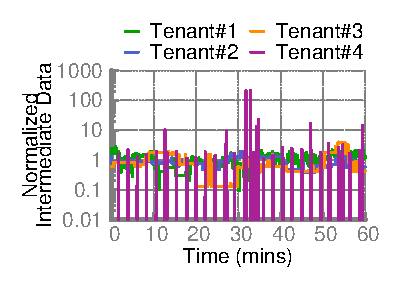
\includegraphics[width = 0.45\textwidth]{fig/jiffy/ephemeral_avg}
    \label{fig:ephemeral-avg}
  }
  \subfigure[\scriptsize Cumulative intermediate data (normalized by peak usage)] {
    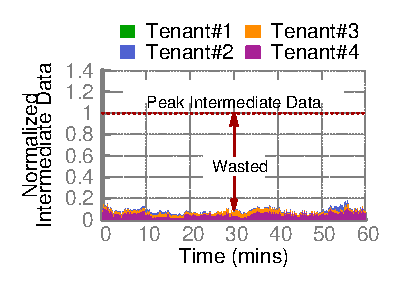
\includegraphics[width = 0.45\textwidth]{fig/jiffy/ephemeral}
    \label{fig:ephemeral-cum}
  }
  \caption[Snowflake workload anaylsis.]{\small{Analysis of production workloads from Snowflake~\cite{snowset} for four tenants over a $1$ hour window: (a) the ratio of peak to average storage usage for a job can vary by an order of magnitude during its execution; and (b) provisioning for peak usage results in average utilization $<10\%$. Across all tenants, the average utilization is $19\%$.}}\label{fig:ephemerals}%\vspace{-1.25em}
\end{figure}


To address this, we start with data analytics applications in serverless computing~\cite{starling, locus, pocket, flint, sparkonlambda, cirrus, excamera, pywren, numpywren, gg, athena, aurora, azuresqldw, cloudburst, snowset, caerus}, a widely adopted workload in modern data centers. Serverless architectures inherently offer on-demand elasticity, decoupling compute and storage resources logically. Recent advances in serverless analytics have demonstrated the benefits of using serverless architectures for resource- and cost-efficient data analytics. In these systems, remote, low-latency, high-throughput disaggregated memory is used to store intermediate states for inter-task{\footnote{Existing distributed programming frameworks, while different in underlying programming models and semantics, share a common structure (Figure~\ref{fig:example}) --- the job is split into multiple {\em tasks}, possibly organized along multiple stages or a directed acyclic graph. Each task generates {\em intermediate} data during its execution; upon completion, each task partitions its intermediate data and exchanges it with tasks in the next stage.}} communication and multi-stage jobs, extending the lifetime of data beyond the task that produced it. This natural separation of compute and memory makes serverless computing an ideal candidate for leveraging disaggregated memory architectures.

As discussed in ~\cite{starling, shuffling, pocket, cirrus}, these applications handle user requests in the form of jobs, each defining its memory needs upon creation. The dilemma of balancing performance with resource efficiency for job-level memory allocation has been extensively studied ~\cite{elasticquery, qoop}. If a job is based on average demand, performance may decline during peak demand periods due to inadequate memory, causing data spillage to slower secondary storage, such as SSDs. Conversely, allocating memory for peak demands leads to underutilization of resources when the actual demand is below peak. Evaluations on Snowflake's workload, as shown in ~\cite{elasticquery}, indicate a significant fluctuation in the ratio of peak to average demands, sometimes varying by two orders of magnitude within minutes.

Designing a memory management service for such systems is a non-trivial task. We begin by outlining the essential requirements for memory management in disaggregated environments, focusing on the unique challenges posed by disaggregation. We then discuss our efforts to address these challenges and suggest potential future directions for research in this rapidly evolving field.

\paragraphb{Elasticity}  Memory usage in modern computing is highly variable, with applications facing fluctuating demands~\cite{jiffy}. Elasticity enables dynamic memory allocation based on current needs, optimizing resource utilization. Applications like data analytics consist of jobs with multiple tasks that communicate via intermediate memory. Traditional solutions allocate memory at the job level, where jobs specify their requirements before execution, and the system reserves that amount for the job's duration~\cite{pocket}. This approach creates a tradeoff: allocating for average demand risks performance degradation due to swapping data to slower storage (e.g., S3), as shown in Figure~\ref{fig:ephemeral-avg}, while allocating for peak demand leads to resource waste (Figure~\ref{fig:ephemeral-cum}). Recent studies report that intermediate data sizes can vary by orders of magnitude during a job's lifetime~\cite{snowset}. For example, Figure~\ref{fig:ephemerals} shows that in a Snowflake dataset with over 2000 tenants, peak-to-average memory demand can vary by two orders of magnitude within minutes, resulting in performance degradation and resource inefficiency in job-level allocations.

\paragraphb{Isolation} The second requirement is the isolation between different compute tasks. Since multiple computing threads can be using the same disaggregated memory pool, it's essential to multiplex between applications to improve resource efficiency but at the same time keep the memory of different threads isolated from each other, which means that the memory usage of a particular application should not affect other existing applications. The number of tasks reading and writing to the shared disaggregated memory can change rapidly in serverless analytics which makes the problem even more severe.

\paragraphb{Lifetime management}
Decoupling compute tasks from their intermediate storage means that the tasks can fail independent of the intermediate data, therefore we need mechanisms for explicity lifetime management of intermediate data.

\paragraphb{Data repartitioning}
Decoupling tasks from their intermediate data also means that data partitioning upon elastic scaling of memory capacity becomes challenging, especially for certain data types used in serverless analytics (e.g. key-value store). If it's the application's responsibility to perform such repartitioning, it will involve large network transfers betweem compute tasks and the far memory system and massive read/write operations every time the capacity is scaled. What's more, the application need to implement different partitioning strategies for different kind of data structures used. Therefore, new mechansims to efficiently enable data partitioning within the far memory system is essential.


We present Jiffy, an elastic disaggregated-memory system for stateful serverless analytics. Jiffy allocates memory resources at the granularity of small fixed-size memory blocks - multiple memory blocks store intermediate data for individual tasks within a job. Jiffy design is motivated by virtual memory design in operating systems that also does memory allocation to individual process at the granularity of fixed-size memory blocks(pages). Jiffy adapts this design to stateful serverless analytics. Performing resource allocation at the granularity of small memory blocks allows Jiffy to elastically scale memory resources allocated to individual jobs without a priori knowledge of intermediate data sizes and to meet the instantaneous job demands at seconds timescales. As a result, Jiffy can efficiently multiplex the available faster memory capacity across concurrently running jobs, thus minimizing the overheads of reads and writes to significantly slower secondary storage (e.g., S3 or disaggregated storage)


\begin{figure}
  \centering
  \begin{tikzpicture}[font=\scriptsize, yscale=0.8, task/.style={draw, circle, align=center, inner sep=2pt}]
    \node[task] (t1) {\texttt{T1}};
    \node[task, above=0.25em of t1] (t2) {\texttt{T2}};
    \node[task, above=0.25em of t2] (t3) {\texttt{T3}};
    \node[task, above=0.25em of t3] (t4) {\texttt{T4}};
    \node[task, right=1.5em of t1, yshift=2em] (t5) {\texttt{T5}};
    \node[task, right=1.5em of t3, yshift=1em] (t6) {\texttt{T6}};
    \node[task, right=4.75em of t3, yshift=-0.5em] (t8) {\texttt{T7}};
    \node[task, right=8em of t2, yshift=-1em] (t10) {\texttt{T8}};
    \node[task, right=8em of t4, yshift=-1em] (t12) {\texttt{T9}};
    
    
    \draw[-stealth] (t1.east) -- (t5.west);
    \draw[-stealth] (t2.east) -- (t5.west);
    \draw[-stealth] (t3.east) -- (t8.west);
    \draw[-stealth] (t4.east) -- (t6.west);
    \draw[-stealth] (t5.east) -- (t8.west);
    \draw[-stealth] (t6.east) -- (t8.west);
    \draw[-stealth] (t8.east) -- (t10.west);
    \draw[-stealth] (t8.east) -- (t12.west);
    
    \node[draw, fill=gray!10, left=2.25em of $(t3)!0.5!(t2)$] {\rotatebox{90}{Persistent Storage}\rotatebox{90}{\quad\quad(\eg, S3)}};
    \node[draw, fill=gray!10, right=11.75em of $(t3)!0.5!(t2)$] {\rotatebox{90}{Persistent Storage}\rotatebox{90}{\quad\quad(\eg, S3)}};
    
    \draw[-stealth] ($(t1.west)+(-1.6em, 0)$) -- (t1.west);
    \draw[-stealth] ($(t2.west)+(-1.6em, 0)$) -- (t2.west);
    \draw[-stealth] ($(t3.west)+(-1.6em, 0)$) -- (t3.west);
    \draw[-stealth] ($(t4.west)+(-1.6em, 0)$) -- (t4.west);
    \draw[-stealth] (t10.east) -- ($(t10.east)+(1.5em, 0)$);
    \draw[-stealth] (t12.east) -- ($(t12.east)+(1.5em, 0)$);
    
    \node[task, above=0.5em of t4, xshift=-1em] (tl) {};
    \node[right=0em of tl] (t) {Task};
    \node[right=2em of t] {Intermediate Data Exchange};
    \draw[-stealth] ($(t)+(2em, 0em)$) -- ($(t)+(3em, 0em)$);
    
  \end{tikzpicture}
  \caption[Execution DAG example for a typical analytics job.]{\small\textbf{Execution DAG example for a typical analytics job.} Intermediate data exchange across tasks occurs via \jiffy.}
  \label{fig:example}
  \label{fig:query-example}
\end{figure}

\section{\jiffy Design}
\label{sec:jiffydesign}

This section explains how \jiffy uses hierarchical addressing, intermediate data lifetime management, and flexible data repartitioning to meet these requirements. We illustrate this with Figure~\ref{fig:query-example}, which depicts the execution plan of a typical analytics job. The plan is represented as a directed acyclic graph (DAG), where nodes are computation tasks (implemented as serverless functions\footnote{Functions refer to basic computation units in serverless architectures, such as Amazon Lambdas~\cite{alambda}, Google Functions~\cite{googlefunctions}, and Azure Functions~\cite{azureFunctions}}), and edges represent intermediate data exchanged via \jiffy.


\begin{figure}[t]
  \centering
  \begin{tikzpicture}[font=\scriptsize, yscale=0.75, task/.style={draw, circle, align=center, inner sep=2pt}, block/.style={draw, align=center, fill=gray!20, inner sep=2pt}]
    \node[task] (t1) {\texttt{T1}};
    \node[task, right=1.5em of t1] (t2) {\texttt{T2}};
    \node[task, right=1.5em of t2] (t3) {\texttt{T3}};
    \node[task, right=1.5em of t3] (t4) {\texttt{T4}};
    \node[task, below=0.5em of t1, xshift=2em] (t5) {\texttt{T5}};
    \node[task, below=0.5em of t4] (t6) {\texttt{T6}};
    \node[task, below=2.75em of t3, xshift=-0.5em] (t8) {\texttt{T7}};
    \node[task, below=5em of t2] (t10) {\texttt{T8}};
    \node[task, below=5em of t4] (t12) {\texttt{T9}};
    
    \node[block, above=0.25em of t3, xshift=-1em] (t3b1) {\texttt{B3\_1}};
    \node[block, above=0.25em of t3, xshift=1em] (t3b2) {\texttt{B3\_2}};
    \node[block, left=0.5em of t5] (t5b1) {\texttt{B5\_1}};
    \node[block, right=0.5em of t6, yshift=0.5em] (t6b1) {\texttt{B6\_1}};
    \node[block, right=0.5em of t6, yshift=-0.5em] (t6b2) {\texttt{B6\_2}};
    \node[block, right=0.5em of t8] (t8b1) {\texttt{B7\_1}};

    \draw[-stealth] (t1.south) -- (t5.north);
    \draw[-stealth] (t2.south) -- (t5.north);
    \draw[-stealth] (t3.south) -- (t8.north);
    \draw[-stealth] (t4.south) -- (t6.north);
    \draw[-stealth] (t5.south) -- (t8.north);
    \draw[-stealth] (t6.south) -- (t8.north);
    \draw[-stealth] (t8.south) -- (t10.north);
    \draw[-stealth] (t8.south) -- (t12.north);
    
    \draw[-stealth] (t3.north) -- (t3b1.south);
    \draw[-stealth] (t3.north) -- (t3b2.south);
    \draw[-stealth] (t5.west) -- (t5b1.east);
    \draw[-stealth] (t6.east) -- (t6b1.west);
    \draw[-stealth] (t6.east) -- (t6b2.west);
    \draw[-stealth] (t8.east) -- (t8b1.west);
    
    \draw[thick, dashed, opacity=0] ($(t5.south west)+(-0.3em, -0.3em)$) rectangle node[midway, right] (t5a) {} ($(t5.north east)+(2.05em, 0.3em)$);
    \draw[thick, dashed, opacity=0, fill=red, fill opacity=0.2] ($(t6.south west)+(-0.3em, -0.75em)$) rectangle node[midway, right] (t6a) {} ($(t6.north east)+(2.75em, 0.75em)$);
    \draw[thick, dashed, opacity=0, fill=red, fill opacity=0.2] ($(t8.south west)+(-0.3em, -0.3em)$) rectangle node[midway, right] (t8a) {} ($(t8.north east)+(2.75em, 0.3em)$);
    
    \node[right=4em of t8a, text width=3em, align=center] (ri) {Task-level Isolation};
    \draw[-stealth, dashed] (ri.west) -- ($(t8a.east)+(1em,0em)$);
    \draw[-stealth, dashed] (ri.north) -- ($(t6a.east)+(1em,0em)$);
    
  \end{tikzpicture}
  \caption[Hierarchical addressing]{\textbf{Hierarchical addressing} for the job in Figure~\ref{fig:query-example}. \jiffy provides task-level resource isolation for ephemeral storage under each task address-prefix (\S\ref{ssec:hva}). Note that block addresses are only assigned to address-prefixes with currently allocated blocks; for tasks \texttt{T1}, \texttt{T2} and \texttt{T4}, blocks are directly read from persistent storage and not stored in \jiffy.}
  \label{fig:hina}
\end{figure}

\subsection{Hierarchical Addressing}
\label{ssec:hva}
Analytics jobs are often structured as multiple stages or a directed acyclic graph (DAG). In serverless analytics, where compute elasticity is key, each job can run tens to thousands of tasks~\cite{starling, locus, pocket, flint, sparkonlambda, cirrus, excamera, pywren, numpywren, gg, athena, aurora, azuresqldw, cloudburst, snowset}. Fine-grained resource allocation requires efficient mapping between tasks and their storage blocks, especially with rapidly changing task concurrency. High concurrency demands task-level isolation, ensuring that task arrival or departure doesn't affect others, avoiding performance degradation.

\jiffy adopts a hierarchical addressing mechanism, inspired by the Internet's IP addressing, to maintain task-to-storage mappings and ensure task-level isolation. \jiffy organizes intermediate data in a virtual address hierarchy based on task dependencies in the DAG. Internal nodes represent tasks, and leaf nodes represent \jiffy blocks storing data. Block addresses are defined by the hierarchy path, with task-generated prefixes. Dependencies between tasks are captured by edges between nodes. \jiffy builds this hierarchy from execution plans (e.g., AWS Step Functions, Azure Durable Functions) or dynamically deduces it via the \jiffy API, supporting dynamic query plans without predefined DAGs.

\paragraphb{Example} Figure~\ref{fig:hina} illustrates the \lh for the job in Figure~\ref{fig:example}. Internal nodes \texttt{T1}-\texttt{T9} represent tasks in the DAG, while leaf nodes \texttt{B3\_1}, \texttt{B3\_2}, etc., represent data blocks allocated by \jiffy for intermediate data storage. Edges like (\texttt{T1}, \texttt{T5}) and (\texttt{T2}, \texttt{T5}) indicate that \texttt{T5} depends on the intermediate data from both \texttt{T1} and \texttt{T2}. The full address of block \texttt{B6\_2} under \texttt{T6} is \texttt{T4.T6.B6\_2}, with \texttt{T4.T6} identifying all blocks under \texttt{T6}. \jiffy constructs the \lh either using the execution plan from Figure~\ref{fig:query-example} or deduces it dynamically. For instance, \sl can infer that since \texttt{T7}'s sub-tasks access data from \texttt{T3}, \texttt{T5}, and \texttt{T6}, these tasks must be its parents in the hierarchy.


By organizing intermediate data in a hierarchy, \jiffy manages resource allocation per address prefix. If one prefix spills to persistent storage (via Pocket), it doesn’t affect others. Blocks remain assigned until reclaimed or leases expire (\S\ref{ssec:mlm}), ensuring task-level isolation regardless of churn. Like virtual memory isolating processes, \jiffy uses hierarchical addressing to isolate tasks based on the job's structure.

Two design considerations arise: (1) \jiffy's fine-grained allocation is independent of fairness policies, which can be layered on top, and (2) address translation from virtual to physical storage happens at a centralized metadata server (like Pocket~\cite{pocket}), scaling to arbitrary DAG sizes. Despite added complexity, \jiffy scales to ${\sim}45$K requests/sec/core, sufficient for most deployments.

\paragraphb{Block sizing} Jiffy balances metadata storage and memory use with block sizes, like $128$MB in HDFS~\cite{hdfs}. Larger blocks reduce metadata but risk fragmentation, while smaller blocks improve utilization at a metadata cost. Jiffy mitigates this via fine-grained access and data repartitioning.

\paragraphb{Isolation granularity} Task-level isolation, where nodes in the hierarchy map to tasks, is default, but finer or coarser isolation (e.g., table-level or stage-level) can be configured via the \jiffy API.


\subsection{Data Lifetime Management}
\label{ssec:mlm}

\begin{figure}[t]
  \centering
  \begin{tikzpicture}[font=\scriptsize, yscale=0.75, task/.style={draw, circle, align=center, inner sep=2pt}, block/.style={draw, align=center, fill=gray!20, inner sep=2pt}]
    \node[task] (t1) {\texttt{T1}};
    \node[task, right=1.5em of t1] (t2) {\texttt{T2}};
    \node[task, fill=BurntOrange!30, right=1.5em of t2] (t3) {\texttt{T3}};
    \node[task, right=1.5em of t3] (t4) {\texttt{T4}};
    \node[task, fill=BurntOrange!30, below=0.5em of t1, xshift=2em] (t5) {\texttt{T5}};
    \node[task, fill=BurntOrange!30, below=0.5em of t4] (t6) {\texttt{T6}};
    \node[task, fill=blue!30, below=2.75em of t3, xshift=-0.5em] (t8) {\texttt{T7}};
    \node[task, fill=BurntOrange!30, below=5em of t2] (t10) {\texttt{T8}};
    \node[task, fill=BurntOrange!30, below=5em of t4] (t12) {\texttt{T9}};
    
    \node[block, fill=BurntOrange!50, above=0.25em of t3, xshift=-1em] (t3b1) {\texttt{B3\_1}};
    \node[block, fill=BurntOrange!50, above=0.25em of t3, xshift=1em] (t3b2) {\texttt{B3\_2}};
    \node[block, fill=BurntOrange!50, left=0.5em of t5] (t5b1) {\texttt{B5\_1}};
    \node[block, fill=BurntOrange!50, right=0.5em of t6, yshift=0.5em] (t6b1) {\texttt{B6\_1}};
    \node[block, fill=BurntOrange!50, right=0.5em of t6, yshift=-0.5em] (t6b2) {\texttt{B6\_2}};
    \node[block, fill=BurntOrange!50, right=0.5em of t8] (t8b1) {\texttt{B7\_1}};

    \draw[-stealth] (t1.south) -- (t5.north);
    \draw[-stealth] (t2.south) -- (t5.north);
    \draw[-stealth] (t3.south) -- (t8.north);
    \draw[-stealth] (t4.south) -- (t6.north);
    \draw[-stealth] (t5.south) -- (t8.north);
    \draw[-stealth] (t6.south) -- (t8.north);
    \draw[-stealth] (t8.south) -- (t10.north);
    \draw[-stealth] (t8.south) -- (t12.north);
    
    \draw[-stealth] (t3.north) -- (t3b1.south);
    \draw[-stealth] (t3.north) -- (t3b2.south);
    \draw[-stealth] (t5.west) -- (t5b1.east);
    \draw[-stealth] (t6.east) -- (t6b1.west);
    \draw[-stealth] (t6.east) -- (t6b2.west);
    \draw[-stealth] (t8.east) -- (t8b1.west);
    
    \draw[thick, dashed, opacity=0] ($(t8.south west)+(-0.3em, -0.3em)$) rectangle node[midway, right] (t8a) {} ($(t8.north east)+(2.05em, 0.3em)$);
%    
    \node[circle, fill=blue!30, right=6em of t8a, yshift=2em] (lr) {};
    \node[right=0em of lr, text width=4em] {Requested lease renewal};
    \node[circle, fill=BurntOrange!30, below=0.75em of lr] (ar) {};
    \node[right=0em of ar, text width=4em] {Automatic lease renewal};
    
  \end{tikzpicture}
  \caption[Lease Renewal via Address Hierarchy]{\textbf{Lease Renewal via Address Hierarchy.} Hierarchical addressing simplifies lease renewal in \jiffy (\S\ref{ssec:mlm}), since lease renewal for an address-prefix automatically implies renewals for all parent and descendent address-prefixes in the hierarchy.}\label{fig:mlm}
\end{figure}

Existing ephemeral storage systems manage data at the job level, reclaiming storage when the job deregisters. In serverless analytics, decoupled task execution and storage can lead to orphaned data. \jiffy addresses this by integrating lease management~\cite{gray1989leases, chubby, dhcplease} with hierarchical addressing for task-level data management. Each address prefix has a lease, and data is retained as long as the lease is renewed. Serverless platforms can trigger lease renewals during task monitoring.

Using the DAG hierarchy, \jiffy renews leases for dependent and ancestor tasks automatically, reducing overhead while preventing orphaned data. This strikes a balance between age-based eviction and explicit resource management, ensuring efficient reassignment of resources upon task or job failure.

\paragraphb{Example} In Figure~\ref{fig:query-example}, task \texttt{T7}'s job periodically renews the lease for the prefix \texttt{T4.T6.T7}\footnote{Task \texttt{T7} has four address prefixes; the job can renew any.}. Renewing \texttt{T7}'s lease also renews those for parent tasks (\texttt{T3}, \texttt{T5}, \texttt{T6}) and descendants (\texttt{T8}, \texttt{T9}), as shown in Figure~\ref{fig:mlm}. This ensures that both parent and descendant tasks' data remain accessible.

\paragraphb{Lease duration} Lease duration trades off control plane bandwidth with system utilization. Longer leases reduce network traffic but may delay resource reclamation. Configuring lease durations, as studied in prior work~\cite{chubby, gray1989leases}, allows \jiffy to meet specific deployment goals.



\subsection{Flexible Data Repartitioning}
\label{ssec:fdr}

Decoupling compute tasks from their intermediate data in serverless analytics poses challenges for achieving fine-grained elasticity in ephemeral storage. Specifically, as storage is allocated or deallocated for a task, the intermediate data must be efficiently repartitioned across the available blocks. However, the decoupling of compute from storage, along with the large number of concurrent tasks, means this repartitioning should not be handled by the application itself. For example, many serverless analytics systems~\cite{locus, pocket} rely on key-value stores for intermediate data. In such cases, if the compute task were responsible for repartitioning during memory scaling, it would need to read key-value pairs over the network, compute new partitions based on the updated memory, and then write the data back to the store—resulting in significant network latency and bandwidth overhead.

\begin{table}[t]
    \centering
    \footnotesize
    \label{table:api}
    \begin{tabular}{c|l}
        \hline
        \textbf{API Group} & \textbf{Function Signature} \\
        \hline
        \multicolumn{1}{c|}{} & connect(honeycombAddress) \\
        \hline
        \multirow{4}{*}{Address Hierarchy} 
            & createAddrPrefix(addr, parent, optionalArgs) \\
            & createHierarchy(dag, optionalArgs) \\
            & flushAddrPrefix(addr, externalPath) \\
            & loadAddrPrefix(addr, externalPath) \\
        \hline
        \multirow{2}{*}{Lease Operations} 
            & leaseDuration = getLeaseDuration(addr) \\
            & renewLease(addr) \\
        \hline
        \multirow{3}{*}{Data Structure}
            & ds = initDataStructure(addr, type) \\
            & listener = ds.subscribe(op) \\
            & notif = listener.get(timeout) \\
        \hline
    \end{tabular}
    \caption[\jiffy User-facing API]{\textbf{\jiffy User-facing API}: Functions for connecting, managing address hierarchies, handling leases, and interacting with data structures.}
\end{table}



\begin{comment}
\begin{table}[t]
	\centering
	\footnotesize
	\caption[\jiffy User-facing API]{\textbf{\jiffy User-facing API}. }
	\label{table:api}
	\begin{tabular}{c|l|l}
		\hline
		\multicolumn{2}{c|}{\textbf{API}} & {\textbf{Description}}\\
		\hline
		\hline
        \multicolumn{1}{c}{} & \begin{lstlisting}[gobble=10]
          connect(JiffyAddress)
        \end{lstlisting} & \specialcell{Connect to \jiffy.}\\\cline{1-3}
        \parbox[t]{2mm}{\vspace{-.75em}\multirow{2}{*}{\rotatebox[origin=c]{90}{\footnotesize Address Hierarchy}}} & \begin{lstlisting}[gobble=10]
          createAddrPrefix(addr, parent, optionalArgs)
          createHierarchy(dag, optionalArgs)
          flushAddrPrefix(addr, externalPath)
          loadAddrPrefix(addr, externalPath)
        \end{lstlisting} &\specialcell{Create address-prefix \texttt{addr} with given \texttt{parent} address-prefix and\\\texttt{optionalArgs} (\eg, initial capacity), or, create address hierarchy\\ from execution plan provided as a DAG \texttt{dag}.\\ Flush/load data in address-prefix to external persistent store.}\\\cline{2-3}
		\multicolumn{1}{c|}{} & \begin{lstlisting}[gobble=10]
          leaseDuration = getLeaseDuration(addr)
          renewLease(addr)
        \end{lstlisting} & \specialcell{Get the lease duration associated with address-prefix \texttt{addr}.\\ Send lease renewal request for address-prefix \texttt{addr}.}\\\cline{1-3}
        \multicolumn{1}{c|}{\parbox[t]{2mm}{\multirow{5}{*}{\rotatebox[origin=l]{90}{\footnotesize Data Structure}}}} & \begin{lstlisting}[gobble=10]
          ds = initDataStructure(addr, type)
        \end{lstlisting} & \specialcell{Initialize data structure of given \texttt{type} in address-prefix \texttt{addr} and\\get handle \texttt{ds} that encapsulates physical locations of allocated blocks.}\\\cline{2-3}
        \multicolumn{1}{c|}{} & \specialcell{\footnotesize Data structure-specific interface implemented using block API (Figure~\ref{fig:blockapi}).} 
          & See Table~\ref{table:ds} in \S\ref{sec:models} for examples. \\\cline{2-3}
        \multicolumn{1}{c|}{} & \begin{lstlisting}[gobble=10]
          listener = ds.subscribe(op)
          notif = listener.get(timeout)
        \end{lstlisting} & \specialcell{Subscribe to notifications for operations of type \texttt{op} on \texttt{ds}.\\Get latest notification; waits \texttt{timeout} seconds for response.}\\\hline
        \hline
	\end{tabular}
\end{table}
\end{comment}

\jiffy supports standard data structures used in data analytics frameworks, including files~\cite{sparkonlambda, athena, aurora, azuresqldw, snowset}, key-value pairs~\cite{pywren, locus, starling, gg, cirrus, cloudburst, pocket, starling}, and queues~\cite{flint, excamera}. Analytics jobs using these structures can offload intermediate data repartitioning during resource allocation or deallocation to \jiffy. Each block in a \jiffy data structure tracks its memory usage. When usage exceeds a high threshold, \jiffy allocates a new block to the corresponding address-prefix\footnote{Similar to existing systems~\cite{elasticache, redis, ramcloud, pocket}, \sl can scale cluster capacity by adding or removing servers based on the number of free blocks. Here, we focus on fine-grained elasticity.}. The overloaded block then triggers data-specific repartitioning to move some of its data to the new block. Conversely, when block usage falls below a low threshold, \jiffy merges it with another low-usage block before deallocating the block. By letting the block, rather than the compute task, handle repartitioning, \jiffy minimizes network and compute overhead for the task. Repartitioning occurs asynchronously, allowing data access to continue with minimal impact on performance.

Jiffy’s supported data structures enable the serverless implementation of powerful distributed frameworks like MapReduce~\cite{mapreduce,spark}, Dryad~\cite{dryad}, StreamScope~\cite{streamscope}, and Piccolo~\cite{piccolo}. Since files, queues, and key-value stores in analytics frameworks require simple repartitioning (unlike complex data structures like B-trees), serverless applications can leverage \jiffy's flexible repartitioning without modification.

\paragraphb{Thresholds for Elastic Scaling} The high and low thresholds in \jiffy balance network bandwidth usage and task performance against system utilization. If thresholds are set too high or low, elastic scaling is triggered infrequently, reducing network traffic but leading to inefficient block utilization (e.g., many nearly empty blocks). Optimal threshold values depend on workload characteristics, as explored in prior work~\cite{mongo-shard, ceph-shard}. \jiffy provides flexibility by exposing these thresholds as configurable parameters, enabling users to tune them according to their needs.

\section{\jiffy Implementation}
\label{sec:jiffyimplementation}

\jiffy builds on Pocket, inheriting its scalable and fault-tolerant metadata plane, multi-tiered data storage, system-wide capacity scaling, and analytics execution model. However, \jiffy introduces hierarchical addressing, lease management, and efficient data repartitioning to address the unique challenges of serverless environments. Below, we describe the \jiffy interface and implementation, highlighting these key features.

\subsection{\jiffy Interface}
\label{ssec:jiffyapi}


We describe \jiffy interface in terms of its user-facing API (Table~\ref{table:api}) and internal API (Figure~\ref{fig:blockapi}).

\paragraphb{User-facing API} The user-facing interface (Table~\ref{table:api}) is built around two core abstractions: \textit{hierarchical addresses} and \textit{data structures}. Jobs can add a new address-prefix using \texttt{createAddrPrefix}, specifying the parent prefix and optional parameters like initial capacity. The \texttt{createHierarchy} interface generates the full hierarchy from an execution plan (DAG), and \texttt{flush}/\texttt{load} allow persistence and retrieval of address-prefix data from external storage (e.g., S3). Three built-in data structures can be associated with an address-prefix via \texttt{initDataStructure}, and new data structures can be defined using the internal API.

Similar to existing systems~\cite{redis, sns}, data structures also expose a notification interface, so that tasks that consume intermediate data can be notified on data availability. For instance, a task can \texttt{subscribe} to write operations on its parent task's data structure, and obtain a \texttt{listener} handle. \jiffy asynchronously notifies the \texttt{listener} upon a write to the data structure, which the task can get via \texttt{listener.get()}.

\begin{figure}[h]
  \centering
  \begin{tabular}{c}
  {\begin{lstlisting}[frame=single, gobble=4, linewidth=20em]
    block = ds.getBlock(op, args) // Get block
    block.writeOp(args) // Perform write
    data = block.readOp(args) // Perform read
    block.deleteOp(args) // Perform delete
  \end{lstlisting}}
  \end{tabular}
  \caption[\jiffy Internal API]{\textbf{\jiffy Internal API.} The block interface is used internally in \jiffy to implement the data structure APIs (\S\ref{sec:models}).}  
  \label{fig:blockapi}
\end{figure}

\paragraphb{Internal API} The data layout within blocks in \jiffy is unique to the data structure that owns it. As such, \jiffy blocks expose a set of data structure \textit{operators} (Figure~\ref{fig:blockapi}) which uniquely defines how data structure requests are \textit{routed} across their blocks, and how data is \textit{accessed} or \textit{modified}. These operators are used internally within \jiffy for its built-in data structures (\S\ref{sec:models}) and not exposed to jobs directly. 

The \texttt{getBlock} operator determines which block an operation request is routed to based on the operation type and operation-specific arguments (\eg, based on key hashes for a KV-store), and returns a handle to the corresponding block. Each \jiffy block exposes \texttt{writeOp}, \texttt{readOp} and \texttt{deleteOp} operators to facilitate data structure-specific access logic (\eg, \texttt{get}, \texttt{put} and \texttt{delete} for KV-store). \jiffy executes individual operators \textit{atomically} using sequence numbers, but does not support atomic transactions that span multiple operators. 

\begin{table*}[t]
  \centering
  \small
  \caption[\jiffy Data Structure Implementations]{\small\textbf{\jiffy Data Structure Implementations}. See \S\ref{sec:models} for details.}
  \label{table:ds}
  \begin{tabular}{c|l|l|l|l|l|l}
        \hline
		\multicolumn{2}{c|}{\multirow{2}{*}{\textbf{Data Structure}}} & \multicolumn{5}{c}{\textbf{Operators}} \\\cline{3-7}
		\multicolumn{2}{c|}{} & \texttt{writeOp} & \texttt{readOp} & \texttt{deleteOp} & \texttt{getBlock} & \texttt{repartition} \\
    	\hline
		\hline
		\parbox[t]{2mm}{\multirow{3}{*}{\rotatebox[origin=c]{90}{\footnotesize Built-in}}} & File (\S\ref{ssec:bsp}) & \texttt{write} & \texttt{read} & \texttt{-} & \specialcell{Route to block based on file offsets.} & Not required \\\cline{2-7}
		& FIFO Queue (\S\ref{ssec:dflow}) & \texttt{enqueue} & \multicolumn{2}{c|}{\texttt{dequeue}} & \specialcell{\texttt{enqueue} to tail, \texttt{dequeue} to head block.} & Not required \\\cline{2-7}
        & KV-Store (\S\ref{ssec:piccolo}) & \texttt{put} & \texttt{get} & \texttt{delete} & \specialcell{Route to block based on key hash.} & Hash-based repartitioning \\\hline
        \multicolumn{7}{c}{Custom data structures.}\\
		\hline
		\hline
  \end{tabular}
\end{table*}
%

\begin{figure}[h]
  \centering
  \begin{tikzpicture}[font=\scriptsize, yscale=0.9, level distance=1.7em, level 1/.style={sibling distance=3em}, level 2/.style={sibling distance=3em}, level 3/.style={sibling distance=3em}]
  	\node (root) [draw, text width=5em, align=center] {Job to address\\prefix mapping}
  	   child { node[fill=gray!10] (app1) {\aa}
        child { node[fill=gray!10] (g1) {\texttt{T1}} 
          child { node[fill=gray!10] (task1) {\texttt{T3}} }
          child { node {...} }
        }
        child { node[fill=gray!10] (g2) {\texttt{T2}} 
          child { node (r) {...} }
        }
      }
      child {
        node[fill=gray!10] (app2) {\ab}
        child { node {...} }
      };
    \draw[black, thick, color=gray] ($(app1.north west)+(-3.25em,2.25em)$) rectangle node[midway, right] (tree-border) {} ($(r.south east)+(2.5em,-0.5em)$);
  	\node[draw, dotted, fill=gray!10, text width=3.5em, align=center, left=0.25em of g1.north west, yshift=1.75em] (internal) {children, permissions, timestamp, blocks, ...};
  	\draw[dotted] ($(g1.north west)+(1em, 0em)$) -- (internal.north east);
  	\draw[dotted] (g1.north west) -- (internal.south east);
  	

    \node[draw, below=0.75em of r.south east, xshift=-2.9em] (head) {};
    \node[draw, right=0.5em of head] (mid1) {};
    \node[draw, right=0.5em of mid1] (mid2) {};
    \node[draw, right=0.5em of mid2] (mid3) {};
    \node[draw, right=0.5em of mid3] (tail) {};

    \draw[-latex] (head.east) -- (mid1.west);
    \draw[-latex] (mid1.east) -- (mid2.west);
    \draw[-latex] (mid2.east) -- (mid3.west);
    \draw[-latex] (mid3.east) -- (tail.west);

    \node[left=-0.25em of head] (flist) {Free List};

    \draw[black, thick, color=gray] ($(flist.north west)+(0.15em, 0em)$) rectangle ($(tail.south east)+(0.2em, -0.25em)$);
  	
  	\node[draw, fill=green!30, text width=5.5em, align=center] (fs-api) at ([xshift=8em, yshift=2.55em]tree-border){$\strut$Metadata Manager};
  	
  	\node[draw, fill=BurntOrange!20, minimum height=4em, text width=5.5em, align=center, below=0.1em of fs-api] (lm) {};
  	\node[text width=5.5em, align=center, below=-0.1em of lm.north] (lm-title) {Lease Manager};
  	\node[draw, fill=BurntOrange!50, text width=5.4em, align=center, below=-0.1em of lm-title] (lm-renewal) {Renewal Service};
  	\node[draw, fill=BurntOrange!50, text width=5.4em, align=center, below=0.1em of lm-renewal] (lm-expiry) {Expiry Worker};
  	
  	\node[draw, fill=blue!30, minimum height=1em, text width=5.5em, align=center, below=0.1em of lm] (sm) {$\strut$Block Allocator};
  	
  	\draw[black, thick, color=gray] ($(app1.north west)+(-6.25em,2.4em)$) rectangle node[midway, right] (dir-border) {} ($(sm.south east)+(0.4em,-0.75em)$);
  	
  	\node[draw, dashed, text width=2.5em, align=center, right=1em of fs-api] (client) {Client};
  	\node[draw, dashed, text width=2.5em, align=center, right=1em of sm] (ss) {Data Plane};
  	
  	\draw[stealth-stealth, thick] (fs-api.east) -- (client.west);
  	\draw[stealth-stealth, thick] (lm-renewal.east) -- (client.west);
  	\draw[stealth-stealth, thick] (sm.east) -- (client.west);
  	\draw[stealth-stealth, thick] (fs-api.east) -- (ss.west);
  	\draw[stealth-stealth, thick] (lm-expiry.east) -- (ss.west);
  	\draw[stealth-stealth, thick] (sm.east) -- (ss.west);
  	
  	\draw[stealth-stealth, thick] (fs-api.west) -- ($(fs-api.west)+(-1em, 0em)$);
  	\draw[stealth-stealth, thick] (lm.west) -- ($(lm.west)+(-1em, 0em)$);
  	\draw[stealth-stealth, thick] ($(sm.west)+(0em,0.5em)$) -- ($(sm.west)+(-1em, 0.5em)$);
    \draw[stealth-stealth, thick] ($(sm.west)+(0em,-0.5em)$) -- ($(sm.west)+(-1em, -0.5em)$);
	
  \end{tikzpicture}
  \caption[\jiffy controller]{\small\textbf{\jiffy controller.} See \S\ref{sec:cp} for details.}
  \label{fig:ds-arch}
\end{figure}
%
\subsection{System Implementation}
\label{sec:cp}
\label{sec:dp}

Since \jiffy design builds on Pocket, its high-level design components are also similar, except for one difference: \jiffy combines the control and metadata planes into a unified control plane. We found this design choice allowed us to significantly simplify interactions between the control and metadata components, without affecting their performance. While this does couple their fault-domains, standard fault-tolerance mechanisms (\eg, the one outlined in~\cite{pocket}) are still applicable to the unified control plane. 


\paragraphb{Control plane} The \jiffy controller (Figure~\ref{fig:ds-arch}) maintains two pieces of system-wide state. First, it stores a \textit{free block list}, which lists the set of blocks that have not been allocated to any job yet, along with their corresponding physical server addresses. Second, it stores an {\lh} per-job, where each node in the hierarchy stores variety of metadata for its address-prefix, including access permissions (for enforcing access control), timestamps (for lease renewal), a block-map (to locate the blocks associated with the address-prefix in the data plane), along with metadata to identify the data structure associated with the address-prefix and how data is partitioned across its blocks. The mapping between jobIDs (which uniquely identify jobs) and their address hierarchies is stored in a hash-table at the controller.

\begin{figure}
  \centering
  \begin{tikzpicture}[font=\scriptsize, yscale=0.7]
    \node[draw, thick, minimum width=4.5em, minimum height=3.25em] (server1) {};
    \node[draw, thick, minimum width=4em, below=0.25em of server1.north] (block11) {};
    \node[fill=gray!40, minimum width=3.675em, inner sep=3pt] at ([xshift=-0.125em]block11) {};
    \node[draw, thick, minimum width=4em, below=0.25em of block11] (block12) {};
    \node[fill=gray!40, minimum width=1.925em, inner sep=3pt] at ([xshift=-1em]block12) {};
    \node[draw, thick, minimum width=4em, below=0.25em of block12] (block13) {};
    \node[fill=gray!40, minimum width=2.925em, inner sep=3pt] at ([xshift=-.5em]block13) {};
    
    \node[text width=4em, align=center, below=0em of server1] {\textbf{Server\#1}};
    
    \node[left=1em of server1] (block) {\textbf{Blocks}};
    \draw[-stealth, thick] (block) -- (block11.west);
    \draw[-stealth, thick] (block) -- (block12.west);
    \draw[-stealth, thick] (block) -- (block13.west);
    
    \draw[thick, dashed] ($(block11.north)+(1.5em, 0.5em)$) -- ($(block13.south)+(1.5em, -1em)$)node [anchor=north] (ht-line) {};
    
    \node[text width=4.5em, align=center, right=0.75em of block13, yshift=-0.5em] (ht) {High threshold};
    
    \draw[-stealth, thick] ($(ht.west)+(0.35em, 0em)$) to [out=225, in=0] (ht-line.north);
    
    \node[draw, thick, minimum width=4.5em, minimum height=3.25em, right=10em of server1] (server2) {};
    \node[draw, thick, minimum width=4em, below=0.25em of server2.north] (block21) {};
    \node[draw, thick, minimum width=4em, below=0.25em of block21] (block22) {};
    \node[fill=gray!40, minimum width=1.925em, inner sep=3pt] at ([xshift=-1em]block22) {};
    \node[draw, thick, minimum width=4em, below=0.25em of block22] (block23) {};
    \node[fill=gray!40, minimum width=1.925em, inner sep=3pt] at ([xshift=-1em]block23) {};
    
    \node[text width=4em, align=center, below=0em of server2] {\textbf{Server\#2}};
    
    \node[draw, thick, dashed, text width=6em, minimum height=1em, align=center, above=3em of $(server1)!0.5!(server2)$] (cp) {\textbf{Control Plane}};
    
    \draw[thick, color=red, -stealth] (block11.north) to [out=90, in=180] node [left, text width=4em, align=center] {\textcolor{red}{\textcircled{1}} Overload signal} (cp.west);
    
    \draw[thick, color=blue, stealth-stealth] (cp.east) to [out=0, in=90] node [right, text width=4em, xshift=0.25em, align=center] {\textcolor{blue}{\textcircled{2}} Allocate \texttt{newBlock}} (block21.north);
    
    \draw[thick, color=violet, -stealth] (cp.south) -- node [right, text width=7em, align=center, yshift=-0.25em] {\textcolor{violet}{\textcircled{3}} \texttt{newBlock} address} ($(block11.east)+(0em, 0.5em)$);
    
    \draw[thick, color=BurntOrange, -stealth] (block11.east) -- node[midway, below, align=center] {\textcolor{BurntOrange}{\textcircled{4}} Repartition data to \texttt{newBlock}} (block21.west);
  \end{tikzpicture}
  \caption[Data repartitioning on scaling up capacity]{\small\textbf{Data repartitioning on scaling up capacity.} Scaling down capacity employs a similar approach (\S\ref{sec:dp}).}\label{fig:autoscaling}
\end{figure}
%
While the block allocator and metadata manager are similar to their counterparts in Pocket, the lease manager implements lifetime management in \jiffy. It comprises a lease renewal service that listens for renewal requests from jobs and updates the lease renewal timestamp of relevant nodes in its \lh, and a lease expiry worker that periodically traverses all address hierarchies, marking nodes with timestamps older than the associated lease period as expired. Finally, \jiffy adopts mechanisms from Pocket to facilitate control plane scaling and fault tolerance; we refer the reader to~\cite{pocket} for details.

\paragraphb{Data plane} \jiffy data plane is responsible for two main tasks: providing jobs with efficient, data-structure specific atomic access to data, and repartitioning data across blocks allocated by the control plane during resource scaling. It partitions the resources in a pool of storage servers across fixed sized blocks. Each storage server maintains, for the blocks managed by it, a mapping from unique blockIDs to pointers to raw storage allocated to the blocks, along with two additional metadata: data structure-specific operator implementations as described in \S\ref{ssec:api}, and a subscription map that maps data structure operations to client handles that have subscribed to receive notifications for that operation. 

Data repartitioning for a \jiffy data structure is implemented as follows: when a block's usage grows above the high threshold, the block sends a signal to the control plane, which, in turn, allocates a new block to the address-prefix and responds to the overloaded block with its location. The overloaded block then repartitions and moves part of its data to the new block (see Figure~\ref{fig:autoscaling}); a similar mechanism is used when the block's usage falls below the low threshold. 

For applications that require fault tolerance and persistence for their intermediate data, \sl supports chain replication~\cite{chainreplication} at block granularity, and synchronously persisting data to external stores (\eg, S3) at address-prefix granularity.


\section{Programming Models on \jiffy}
\label{sec:jiffymodels}

We now describe how \jiffy's built-in data structures (Table~\ref{table:ds}) 
enable many distributed programming frameworks atop serverless platforms 
(\S\ref{ssec:bsp}-\S\ref{ssec:piccolo}). 


\subsection{Map-Reduce Model}
\label{ssec:bsp}

A Map-Reduce (MR) program~\cite{mapreduce} comprises map
functions that process a series of input key-value (KV) pairs 
to generate intermediate KV pairs, and reduce functions that merge 
all intermediate values for the same intermediate key. MR 
frameworks~\cite{mapreduce, hadoop, spark} parallelize map and reduce 
functions across multiple workers. Data exchange between
map and reduce workers occurs via a shuffle phase, where intermediate
KV pairs are distributed in a way that ensures values belonging
to the same key are routed to the same worker.

MR on \jiffy executes map/reduce tasks as serverless tasks. A
master process launches, tracks progress of, and handles failures for 
tasks across MR jobs. \sl stores intermediate
KV pairs across multiple shuffle files, where
shuffle files contain a partitioned subset of KV pairs
collected from all map tasks. Since multiple map tasks can 
write to the same shuffle file, \jiffy's strong consistency 
semantics ensures correctness. The master 
process handles explicit lease renewals. We describe \jiffy files next.

\paragraphb{\jiffy Files} A \jiffy file is a collection of blocks, each storing a fixed-sized chunk of the file. 
The controller stores the mapping between blocks and
file offset ranges managed by them at the metadata manager;
this mapping is cached at clients accessing the file, and updated
whenever the number of blocks allocated to the file is scaled in \jiffy.
The \texttt{getBlock} operator forwards requests to different file blocks 
based on the offset-range for the request.
Files support sequential \texttt{read}s, and \texttt{write}s via 
append-only semantics. For random access, 
files support \texttt{seek} with arbitrary offsets. 
\jiffy uses the provided offset to identify the corresponding 
block, and forwards subsequent \texttt{read}
requests to it. Finally, since files are append-only, blocks 
can only be added to it (not removed), and do not require 
repartitioning when new blocks are added. 

\subsection{Dataflow and Streaming Dataflow Models}
\label{ssec:dflow}

In the dataflow programming model, programmers provide DAGs to describe 
an application's communication patterns. DAG vertices correspond to computations,
while data channels form directed edges between them. We use
Dryad~\cite{dryad} as a reference dataflow execution engine, where 
channels can be files, shared memory FIFO queues, \etc~Dryad runtime 
schedules DAG vertices across multiple workers based on their 
dataflow dependencies. A vertex is scheduled when 
all its input channels are ready: a file channel is ready if all its data 
items have been written, while a queue is ready if it has any data item. 
Streaming dataflow~\cite{streamscope} employs a similar
approach, except channels are continuous event streams.

Dataflow on \jiffy maps each DAG vertex to a serverless task,
while a master process handles vertex scheduling,
fault tolerance, and lease renewals for task address-prefixes. We use \sl FIFO
queues and files as data channels. Since queue-based channels are considered 
ready as long as some vertex is writing to it, \sl allows downstream tasks 
to efficiently detect availability of items produced by upstream tasks 
via notifications, as described below.

\paragraphb{\jiffy Queues} The FIFO queue in \jiffy is a continuously growing linked-list of blocks, where each block stores multiple data items, and a pointer to the next block in the list. The queue size can be upper-bounded (in number of items) by specifying a \texttt{maxQueueLength}. The controller only stores the head and the tail blocks in the queue's linked list, which the client caches and updates whenever blocks are added/removed. The FIFO queue supports \texttt{enqueue}/\texttt{dequeue} to add/remove items. The \texttt{getBlock} operator routes \texttt{enqueue} and \texttt{dequeue} operations to the current tail and head blocks in the link-list, respectively. While, blocks can be both added and removed from a FIFO queue, queues do not need subsequent data repartitioning. Finally, the FIFO queue leverages \jiffy notifications to asynchronously detect when the there is data in the queue to consume, or space in the queue to add more items via subscriptions to \texttt{enqueue} and \texttt{dequeue}, respectively. 


\subsection{Piccolo}
\label{ssec:piccolo}

Piccolo~\cite{piccolo} is a data-centric programming model that allows
distributed compute machines to share distributed,
mutable state. Piccolo
kernel functions specify sequential application logic and share
state with concurrent kernel functions via a KV
interface, while centralized control functions create and coordinate both shared
KV stores and kernel function instances. Concurrent updates to 
the same key in the KV store are resolved using 
user-defined accumulators. 

Piccolo on \jiffy runs kernel functions across serverless tasks, while
control tasks run on a centralized master. The shared
state is stored across \sl's KV-store data 
structures (described below). KV-stores may be created per kernel function, 
or shared across multiple functions, depending on the application needs. 
The master periodically renews 
leases for \sl KV-stores. Like Piccolo,
\sl checkpoints KV-stores by flushing them to an external 
store.

\paragraphb{\jiffy KV-store} The \sl KV-store hashes each key to one of $H$ hash-slots in the range $[0,H$-$1]$ ($H$=$1024$ by default). The KV-store shards KV pairs across multiple \jiffy blocks, such that each block owns one or more hash-slots in this range. Note that a hash-slot is completely contained in a single block. The controller stores the mapping between the blocks and the hash slots managed by them; this metadata is, again, cached at the client and updated during resource scaling. Each block stores KV pairs that hash to its slots as a hash-table. The KV-store supports typical \texttt{get}, \texttt{put}, and \texttt{delete} operations as implementations of \texttt{readOp}, \texttt{writeOp} and \texttt{deleteOp} operators. The \texttt{getBlock} operator routes requests to KV-store blocks based on key-hashes. 

Unlike files and queues, data needs to repartitioned for the KV-store when a block is added or removed. When a block is close-to-full, \jiffy reassigns half of its hash-slots to a new block, moves the corresponding key-value pairs to it, and updates the block-to-hash-slot mapping at the controller. Similarly, when a block is nearly empty, its hash-slots are merged with another block. 



\section{Evaluation}
\label{sec:jiffyevaluation}
\jiffy is implemented in $25$K lines of C++, with client libraries in C++, Python and Java (${\sim}1$K LOC each); this is in addition to the original Pocket code. In this section, we evaluate \jiffy to demonstrate its benefits (\S\ref{ssec:overallbenefits}, \S\ref{ssec:hrelated}) and to understand the contribution of individual \jiffy mechanisms to its overall performance (\S\ref{ssec:benefits}). Finally, we evaluate \jiffy controller overheads in \S\ref{ssec:controller-scale}.

\paragraphb{Experimental setup} Unless otherwise specified, each intermediate storage system in our experiments is deployed across $10$ m4.16xlarge EC2~\cite{ec2} instances, while serverless applications are deployed across AWS Lambda~\cite{ec2} instances. Since \jiffy builds on Pocket design, it supports addition of new instances to increase the system-wide capacity. However, our experiments do not evaluate overheads for doing so, since, it is orthogonal to \jiffy's goals; we specifically focus on multiplexing available system storage capacity for higher utilization and reducing the need for adding more capacity. \jiffy employs $128$MB blocks, $1$s lease duration and $5\%$ (low) and $95\%$ (high) as thresholds for data repartitioning. 

\begin{figure}[t]
  \centering
  \subfigure[Job performance] {
    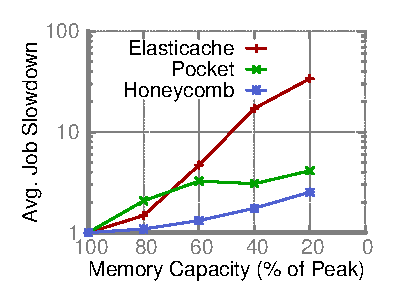
\includegraphics[width = 1.54in]{fig/jiffy/perfvcap}
    \label{fig:perfvcap}
  }
  \subfigure[Resource utilization] {
    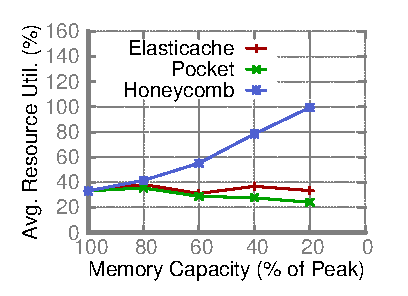
\includegraphics[width = 1.54in]{fig/jiffy/utilvcap}
    \label{fig:utilization}
  }
  \caption[Fine-grained task-level elasticity in \jiffy]{\textbf{Fine-grained task-level elasticity in \jiffy} enables (a) better job performance, and (b) higher resource utilization under constrained capacity. In (a), the slowdown is computed relative to the job completion time with $100\%$ capacity (for this data point, Elasticache performance was $30\%$ worse than Pocket, and Pocket performance was $5\%$ worse than \jiffy). See \S\ref{ssec:overallbenefits} for details.}
  \label{fig:elasticity}\vspace{-1.25em}
\end{figure}


\subsection{Benefits of \jiffy}
\label{ssec:overallbenefits}

\jiffy enables fine-grained resource allocation for serverless analytics. We demonstrate the benefits of this approach to job performance and resource utilization for roughly $50,000$ jobs across $100$ randomly chosen tenants over a randomly selected $5$ hour window in the Snowflake workload\footnote{{We were unable to evaluate the entire $14$ day window with $>2000$ tenants due to intractable cost overheads.}}~\cite{snowset}. 

We compare \jiffy (with the MR programming model, \S\ref{sec:models}) against Elasticache~\cite{elasticache} and Pocket~\cite{pocket}. Elasticache represents systems that provision resources for \textit{all} jobs. Since Elasticache does not support multiple storage tiers, if available capacity is insufficient, jobs must write their data to external stores like S3~\cite{s3}. Pocket, on the other hand, reserves and reclaims resources at \textit{job} granularity; if available capacity is insufficient, Pocket allocates resources on secondary storage (SSD). Note that Pocket's utilization can sometimes be \textit{lower} than Elasticache, since it provisions for the peak of each job \textit{separately}, sacrificing utilization for job-level isolation. Finally, our evaluation for Pocket places its control and metadata services on the same server to ensure a fair comparison with \jiffy's unified control plane.

\paragraphb{Impact of fine-grained elasticity on job performance} We demonstrate this impact by constraining the amount of available capacity at the intermediate store for the Snowflake workload. Figure~\ref{fig:perfvcap} shows the average job slowdown as the capacity is reduced to a certain percentage of the peak utilization for the workload within the evaluated time window (\ie, across all jobs). With Elasticache, job performance suffers significantly when the intermediate data grows larger than capacity ($34\times$ slowdown at $20$\% capacity), since the data must now be accessed from S3. With Pocket, the data spills to SSD when the allocated capacity at the DRAM-tier (during job registration) is insufficient. While the slowdown is less severe due to its efficient tiered-storage, jobs still experience a $>4.1\times$ slowdown at $20$\% capacity. Finally, \jiffy observes much lower job performance degradation with constrained capacity ($<2.5\times$ at $20$\% capacity). This is because task-level elasticity and lease based reclamation of faster storage capacity allows \jiffy to efficiently multiplex capacity across multiple jobs at a much finer granularity than Pocket. This, in turn, significantly reduces data spilling over to a slower storage tier in \jiffy compared to Pocket. We confirm this intuition further by studying the impact of fine-grained elasticity on resource utilization next. 

\paragraphb{Impact of fine-grained elasticity on resource utilization} Figure~\ref{fig:utilization} shows the resource utilization across the compared systems under constrained capacity. While the resource utilization for Elasticache and Pocket either decreases or remains the same as the system capacity is reduced, resource utilization \textit{improves} for \jiffy. This is because Pocket and Elasticache provision capacity (at job or coarser granularity), and the unused capacity is wasted, regardless of the total system capacity. In contrast, \jiffy is able to better multiplex the available capacity across various jobs owing to its fine-grained elasticity and lease-based reclamation of unused capacity. By making better use of available capacity, \jiffy ensures that a much smaller fraction of data spills over to SSD, resulting in better performance in Figure~\ref{fig:perfvcap}.


\begin{figure}
  \centering
  \subfigure[Latency] {
    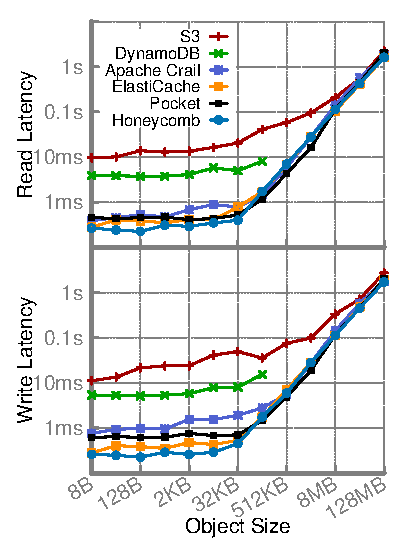
\includegraphics[width = 1.4in]{fig/jiffy/rw_latency}
    \label{fig:rwlatency}
  }%
  \subfigure[MBPS] {
    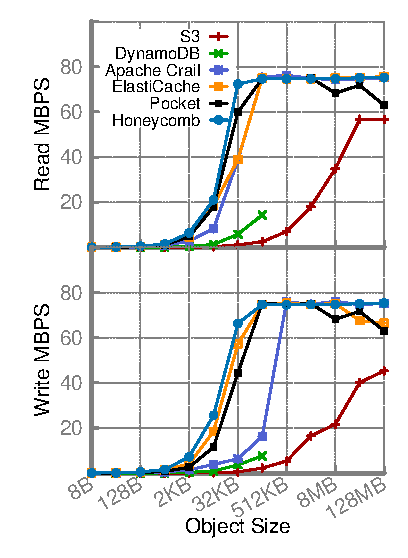
\includegraphics[width = 1.4in]{fig/jiffy/rw_mbps}
    \label{fig:rwmbps}
  }%
  \caption[\jiffy performance comparison with existing storage systems]{\small{\textbf{\jiffy performance comparison with existing storage systems (\S\ref{ssec:hrelated}).} Despite providing the additional benefits demonstrated in \S\ref{ssec:overallbenefits}, \jiffy performs as well as or outperforms state-of-the-art storage systems for serverless analytics.}}
  \label{fig:storage-perf}
\end{figure}

\subsection{Performance Benchmarks for Six Systems}
\label{ssec:hrelated}

We now compare \jiffy performance (using its KV-Store data structure) against five state-of-the-art systems commonly used for intermediate data storage in serverless analytics: S3, DynamoDB, Elasticache, Apache Crail and Pocket. Since only a subset of the compared systems support request pipelining, we disable pipelining for all of them. 



To measure latency and throughput for the above systems, we profiled synchronous operations issued from an AWS Lambda instance using a single-threaded client. Figure~\ref{fig:storage-perf} shows that in-memory data stores like Elasticache, Pocket and Apache Crail achieve low-latency (sub-millisecond) and high-throughput. In contrast, persistent data stores like S3 and DynamoDB observe significantly higher latencies and lower throughput; note that DynamoDB only supports objects up to $128$KB. \jiffy matches the performance achieved by state-of-the-art in-memory data stores, while additionally providing the benefits outlined in \S\ref{ssec:overallbenefits}.


\subsection{Understanding \jiffy Benefits}
\label{ssec:jiffybenefits}

Figure~\ref{fig:elasticity} already shows how fine-grained elasticity in \jiffy allows it to achieve performance and resource utilization gains over the compared state-of-the-art systems. As noted earlier, this fine-grained elasticity is enabled by hierarchical virtual addressing combined with with flexible data lifetime management and data repartitioning in \jiffy. In this section, we evaluate their impact in isolation.

\begin{figure*}[t]
  \centering
  \subfigure[Efficient lifetime management] {
    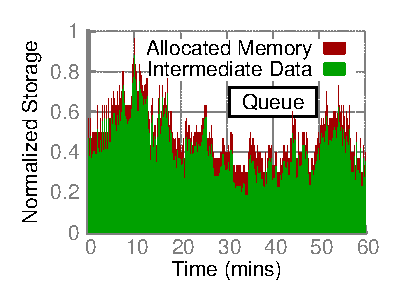
\includegraphics[width = 1.4in]{fig/jiffy/fifo_queue_scale_uniform}\hspace{-.5em}%
    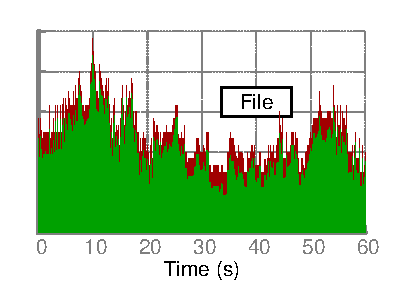
\includegraphics[width = 1.4in]{fig/jiffy/file_scale_uniform}\hspace{-.5em}%
    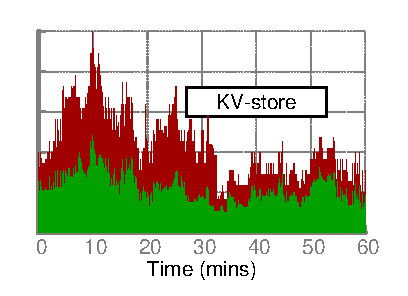
\includegraphics[width = 1.4in]{fig/jiffy/scale_zipf}
    \label{fig:fi-scale}
    \label{fig:ht-scale}
    \label{fig:fq-scale}
  }%
  \subfigure[Efficient data repartitioning] {
    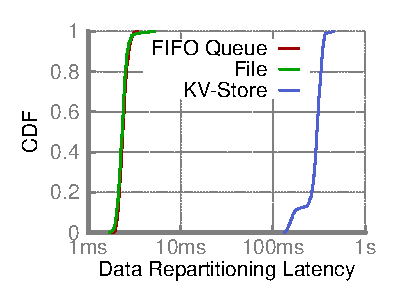
\includegraphics[width = 1.325in]{fig/jiffy/scale_latency_cdf}\hspace{-1.5em}%
    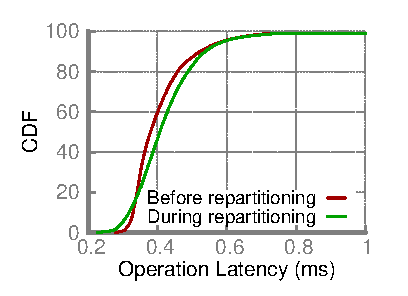
\includegraphics[width = 1.325in]{fig/jiffy/hash_table_scaling_get}
    \label{fig:op-latency-scaling}
    \label{fig:scale-latency}
  }
  \caption[\jiffy data lifetime-management and data repartitioning]{\textbf{\jiffy data lifetime-management and data repartitioning.} (a) \jiffy enables fine-grained elasticity via lease-based lifetime management for its built-in data structures, FIFO Queue (left), File (center) and KV-store (right), reclaiming resources from tasks as soon as their leases expire. (b) \jiffy facilitates efficient data repartitioning for its data structures when their allocation is scaled up, with repartitioning for a single block completing in $2$-$500$ms (left). Moreover, \jiffy latency for 100KB \texttt{get}s is minimally impacted during KV-store repartitioning. Note: plots in (a), (b) share a common y-axis; x-axis for (c, left) is in log-scale.}
\end{figure*}



\paragraphb{Fine-grained elasticity via data lifetime management} Unlike traditional storage systems, \jiffy's lease-based data lifetime management allows it to reclaim unused resources from jobs, and potentially assign them to other jobs that might need them. Coupled with fine-grained resource allocations and efficient data repartitioning, this enables fine-grained elasticity for serverless jobs running on \jiffy. To understand how, we evaluate storage allocation across different \jiffy data structures (Figure~\ref{fig:fq-scale}) when subjected to Snowflake workload from Figure~\ref{fig:ephemerals}.

FIFO queue and file observe seamless elasticity in allocated resources as intermediate data is written to them since they do not require repartitioning. The allocated capacity exceeds the intermediate data size for the data structures by only a small amount; this accounts for the additional metadata stored at each of the blocks (\eg, object metadata for the items enqueued in the FIFO queue, etc.), along with unused space within the head/tail blocks. For the KV-store, the inserted keys were sampled from a Zipf distribution over the keyspace since the Snowflake dataset does not provide access patterns. Due to the skew, a few \jiffy blocks receive most of the key-value pairs, and repeatedly split across newly allocated blocks when their used capacity grows too high. The allocated capacity is therefore higher than the dataset size, since the used capacity is low for most blocks owing to the Zipf key sampling; this corresponds to the worst-case for the KV-Store. However, \jiffy's lease mechanism reclaims resources allocated to the data structures soon after their utility is over, ensuring that the overheads are short-lived. %\rc{Need to talk about Zipf distribution?}


\paragraphb{Efficient elastic scaling via flexible data repartitioning} A key contributor for the fine-grained resource elasticity achieved by \jiffy is its flexible but efficient data repartitioning approach. Figure~\ref{fig:scale-latency} shows the CDF of data repartitioning latency per block across the three data structures, when subjected to the Snowflake workload from above. The data repartitioning latency shown here corresponds to the total time taken from the detection of an overloaded/underloaded block to the end of data repartitioning. The storage server takes ${\sim}1$-$1.5$ms to connect to the controller, and two round-trips ($100$-$200\mu$s in EC2) to trigger allocation/reclamation of data blocks and update for partitioning metadata at the controller. Unlike FIFO Queue and File, KV-Store also requires repartitioning data across blocks. However, since repartitioning a single block only requires moving only half the block capacity (${\sim}64$MB), \jiffy is able to repartition the data in a few hundred milliseconds over $10$Gbps links. As such, \jiffy repartitions data within a block for its built-in data structures with very low latency ($2$-$500$ms).

Finally, we also note that \jiffy does not block data structure operations during data repartitioning. In fact, these operations are minimally impacted during this period: Figure~\ref{fig:op-latency-scaling} shows that the CDF for 100KB \texttt{get} operations on the KV-Store prior to and during scaling are almost identical.

\begin{figure}[h]
  \centering
  \subfigure[Controller throughput vs. latency on a single CPU core.] { 
    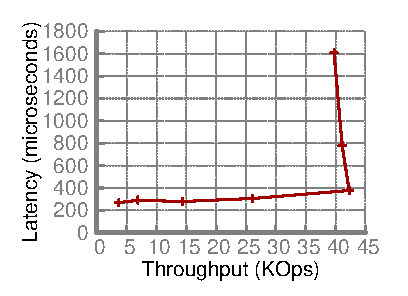
\includegraphics[width = 1.5in]{fig/jiffy/controller_tvl}
    \label{fig:controller-tvl}
  }
  \subfigure[Controller throughput scaling with multiple cores.] {
    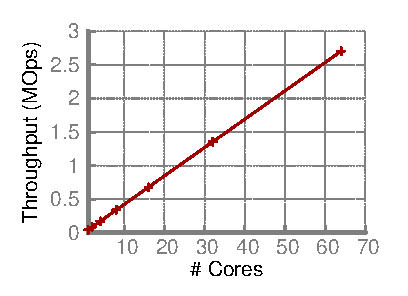
\includegraphics[width = 1.5in]{fig/jiffy/controller_scale}
    \label{fig:controller-scaling}
  }
  \caption[\jiffy controller performance]{{\textbf{\jiffy controller performance.} Details in Appendix~\ref{ssec:controller-scale}.}}
  \label{fig:controller-perf}
\end{figure}

\subsection{Controller Overheads}
\label{ssec:controller-scale}

\jiffy adds several components at the controller compared to Pocket, including all of metadata management, lease management and handling requests for data repartitioning. As such, we expect its performance to be lower than Pocket's metadata server. We deem this to be acceptable as long as it can still handle control plane request rates typically seen for real world workload, \eg, a peak of a few hundred requests per second, including lease renewal requests, for all of our evaluated workloads and those evaluated in~\cite{pocket}.

Figure~\ref{fig:controller-tvl} shows the throughput-vs-latency curve for \jiffy controller operations on a single CPU core of an m4.16xlarge EC2 instance. The controller throughput saturates at roughly $42$ KOps, with a latency of $370$us. While this throughput is lower than Pocket ($\sim 90$KOps per core), it is more than sufficient to handle control plane load for real-world workloads. In addition, the throughput scales almost linearly with the number of cores, since each core can handle requests independent of other cores for a distinct subset of virtual address hierarchies (Figure~\ref{fig:controller-scaling}). Finally, the control plane readily scales to multiple servers by partitioning the set of address hierarchies across them.

\paragraphb{Storage overheads} The task-level metadata storage in Honeycomb has an overhead of only $64$ bytes of fixed metadata per task and $8$ bytes per block. For the default $128$MB blocks used in \jiffy, the metadata storage overhead is a tiny fraction of the total storage ($<0.00005-0.0001\%$).










% ======================================================================

%\section{Introduction}
%
%
%Serverless architectures offer flexible compute and storage options, charging users for precise resource usage. Initially used for web microservices, IoT, and ETL tasks, recent advancements show their efficacy in data analytics. Serverless analytics leverage remote, high-throughput memory systems for inter-task communication and storing intermediate data. However, existing far-memory systems face limitations, allocating resources at the job level, leading to performance issues and underutilization.
%
%To address this, we introduce Jiffy, an elastic far-memory system for stateful serverless analytics. Unlike conventional systems, Jiffy allocates memory in small, fixed-size blocks, enabling dynamic scaling and efficient resource utilization. This approach resolves challenges unique to serverless analytics, including task mapping, task isolation, and data lifetime management.
%
%Our implementation of Jiffy features an intuitive API for seamless data manipulation. We demonstrate its versatility by implementing popular distributed frameworks like MapReduce, Dryad, StreamScope, and Piccolo. Evaluation against state-of-the-art systems indicates Jiffy’s superior resource utilization and application performance, achieving up to 3x better efficiency and 1.6–2.5x performance improvements.
%
%
%\section{Motivation}
%The leading system for stateful serverless analytics is Pocket, a distributed system designed for high-throughput, low-latency storage of intermediate data. Pocket effectively tackles several key challenges in stateful serverless analytics, including:
%
%\paragraphb{Centralized management} Pocket's architecture features separate control, metadata, and data planes. While data storage is distributed across multiple servers, management functions are centralized, simplifying resource allocation and storage organization. A single metadata server can handle significant request loads, supporting thousands of serverless tasks.
%
%\paragraphb{Multi-tiered data storage} Pocket's data plane stores job data across multiple servers and serves them via a key-value API. It supports storage across different tiers like DRAM, Flash, or HDD, enabling flexibility based on performance and cost constraints.
%
%\paragraphb{Dynamic resource management} Pocket can scale memory capacity by adding or removing memory servers based on demand. The controller allocates resources for jobs and informs the metadata plane for proper data placement.
%
%\paragraphb{Analytics execution with Pocket} Jobs interact with Pocket by registering with the control plane, specifying memory resources needed. The controller allocates resources and informs the metadata plane. Serverless tasks can access data directly from memory servers. Once a job finishes, it deregisters to release resources.
%
%In our analysis, we focus on challenges in Pocket's resource allocation. Pocket allocates memory at the job level, which poses challenges in accurately predicting intermediate data sizes and leads to performance degradation or resource underutilization. This issue persists due to the dynamic nature of intermediate data sizes across different stages of execution.
%
%
%\section{Jiffy Design}
%
%Jiffy facilitates precise sharing of far-memory capacity among concurrent serverless analytics tasks for intermediate data storage. Drawing inspiration from virtual memory, Jiffy divides memory capacity into fixed-sized blocks, akin to virtual memory pages, and performs allocations at this granular level. This approach yields two key benefits: firstly, Jiffy can swiftly adapt to instantaneous job demands, adjusting capacity at the block level within seconds. Secondly, Jiffy doesn't necessitate prior knowledge of intermediate data sizes from jobs; instead, it dynamically manages resources as tasks write or delete data.
%
%It's worth noting that multiplexing available memory capacity differs from merely scaling the memory pool's overall capacity. While prior systems like Pocket focus on the latter, adding or removing memory servers based on job arrivals or completions, Jiffy prioritizes efficient sharing of available capacity among concurrent jobs. This approach minimizes underutilization of existing capacity, a common issue in job-level resource allocation systems. Even during high memory capacity utilization, Jiffy can augment capacity by adding memory servers akin to Pocket. Notably, by efficiently multiplexing capacity across concurrent jobs, Jiffy reduces the need for frequent additions or removals of memory servers.
%
%In addressing the challenges posed by serverless analytics, Jiffy implements hierarchical addressing, data lifetime management, and flexible data repartitioning. These mechanisms are discussed in detail in subsequent sections, with illustrative examples provided in Fig. 3, depicting a typical analytics job's execution plan organized as a directed acyclic graph (DAG) with computation tasks represented as serverless functions exchanging intermediate data via Jiffy.
%\subsection{Hierarchical Addressing}
%
%Analytics jobs typically follow a multi-stage or directed acyclic graph structure. In serverless analytics, where compute elasticity is integral, each job may entail tens to thousands of individual tasks. Consequently, achieving fine-grained resource allocation necessitates an efficient mechanism for maintaining an updated mapping between tasks and allocated memory blocks. Additionally, the rapidly changing number of tasks accessing shared memory underscores the importance of isolation at the task level to prevent performance degradation across jobs. In this context, Jiffy's hierarchical addressing system plays a crucial role.
%
%Instead of relying on a network structure, Jiffy employs a hierarchical addressing mechanism tailored to the execution structure of analytics jobs. It organizes intermediate data within a virtual address hierarchy, reflecting the dependencies between tasks in the job's DAG. For instance, internal nodes represent tasks, while leaf nodes denote memory blocks storing intermediate data. The addressing scheme enables precise resource allocation at the task level, independent of other tasks, akin to virtual memory's process-level isolation.
%
%This hierarchical addressing facilitates efficient management of resource allocations, ensuring that overflow into persistent storage doesn't impact the performance of other tasks. Each memory block, once allocated, remains dedicated to its task until explicitly released, guaranteeing isolation at the task level regardless of concurrency. This approach aligns with virtual memory principles, where each process enjoys its own address space, ensuring isolation at the process level.
%
%Jiffy's design considers two key aspects. Firstly, resource allocation is decoupled from policy enforcement, allowing seamless integration of fairness algorithms atop Jiffy's allocation mechanism. Secondly, address translation, handled centrally, enables addressing for arbitrary DAGs without imposing limitations on execution structure complexity. While Jiffy's hierarchical addressing introduces complexity at the controller, its scalability is validated in our evaluation, accommodating realistic deployment demands.
%
%Regarding block sizing, Jiffy's approach, akin to traditional virtual memory's page sizing, balances metadata overhead and memory utilization. Larger block sizes reduce per-block metadata, but may lead to data fragmentation, while smaller sizes optimize memory utilization at the expense of increased metadata overhead. Jiffy mitigates fragmentation via data repartitioning and allows block size configuration during initialization for compatibility with analytics frameworks.
%
%Isolation granularity in Jiffy is task-level by default, but can be adjusted finer or coarser by adapting the hierarchy. For most analytics frameworks, task-level isolation suffices, but custom hierarchies can be created using Jiffy's API to tailor isolation to specific needs.
%
%\subsection{Data Lifetime Management}
%Existing far-memory systems for serverless analytics typically manage data lifetimes at the granularity of entire jobs, reclaiming storage only when a job explicitly deregisters. However, in serverless analytics, the intermediate data of a task is dissociated from its execution, residing in the far-memory system. This decoupling extends to fault domains: traditional mechanisms, such as reference counting, can result in dangling intermediate data if a task fails. To address this inefficiency, effective task-level data lifetime management mechanisms are required.
%
%Jiffy tackles this challenge by integrating lease management mechanisms with hierarchical addressing. Each address-prefix in a job's hierarchical addressing is associated with a lease, and data remains in memory only as long as the lease is renewed. Consequently, jobs periodically renew leases for the address-prefixes of running tasks. Jiffy tracks lease renewal times for each node in the address hierarchy, updating them accordingly. Upon lease expiry, Jiffy reclaims allocated memory after flushing data to persistent storage, ensuring data integrity even in the event of network delays.
%
%A novel aspect of Jiffy's lease management is its utilization of DAG-based hierarchical addressing to determine dependencies between leases. When a task renews its lease, Jiffy extends the renewal to the prefixes of tasks it depends on (parent nodes) and the prefixes of tasks dependent on it (descendant nodes), minimizing the number of renewal messages sent. This approach ensures that not only is a task's own data retained in memory while it's active, but also the data of tasks it depends on and tasks dependent on it. This mechanism strikes a balance between age-based eviction and explicit resource management, granting jobs control over resource lifetimes while tying resource fate to job status.
%
%In an example scenario, task T7 periodically renews leases for its prefix during execution, ensuring the retention of intermediate data for blocks under it in memory. Lease renewals for T7's prefix also extend to its parent and descendant tasks, ensuring continuity of data access. However, leases for inactive tasks are not automatically renewed, preventing unnecessary resource retention.
%
%Lease duration in Jiffy involves a tradeoff between control plane bandwidth and system utilization. Longer lease durations reduce network traffic but may lead to underutilization of resources until leases expire. Jiffy's sensitivity to lease durations is evaluated in the subsequent section.
%
%
%
%
%\subsection{Flexible Data Repartitioning}
%Decoupling compute tasks from their intermediate data in serverless analytics poses a challenge in achieving memory elasticity efficiently at fine granularities. When memory is allocated or deallocated to a task, repartitioning the intermediate data across the remaining memory blocks becomes necessary. However, due to the decoupling and the high concurrency of tasks, it's impractical to expect the application to handle this repartitioning. For instance, in many existing serverless analytics systems, key-value stores are used to store intermediate data. If a compute task were to handle repartitioning upon memory scaling, it would need to fetch key-value pairs from the store over the network, compute new data partitions, and then write back the data, incurring significant network latency and bandwidth overheads.
%
%As discussed in §5, Jiffy already incorporates standard data structures utilized in data analytics frameworks, ranging from files to key-value pairs to queues. Analytics jobs leveraging these data structures can delegate repartitioning of intermediate data upon resource allocation/deallocation to Jiffy. Each block allocated to a Jiffy data structure monitors the fraction of memory capacity currently utilized for data storage. When usage surpasses a high threshold, Jiffy allocates a new block to the corresponding address-prefix. Subsequently, the overloaded block initiates data structure-specific repartitioning to migrate some data to the new block. Conversely, when block usage falls below a low threshold, Jiffy identifies another block with low usage within the address-prefix for potential data merging. The block then undergoes the necessary repartitioning before deallocation by Jiffy.
%
%By tasking the target block with repartitioning instead of the compute task, Jiffy circumvents network and computational overheads for the task itself. Furthermore, data repartitioning in Jiffy occurs asynchronously, enabling data access operations across data structure blocks to proceed even during repartitioning. This ensures minimal impact on application performance due to repartitioning.
%
%The data structures integrated into Jiffy enable the implementation of serverless versions of various powerful distributed programming frameworks, including MapReduce, Dryad, StreamScope, and Piccolo. Notably, the simplicity of repartitioning mechanisms required by analytics framework data structures allows serverless applications utilizing these programming models to seamlessly run on Jiffy and leverage its adaptable data repartitioning without any modifications.
%
%Regarding thresholds for elastic scaling, the high and low thresholds in Jiffy present a tradeoff between data plane network bandwidth and task performance on one side and system utilization on the other. Optimizing these thresholds balances the frequency of elastic scaling triggers and system utilization efficiency. We evaluate Jiffy's sensitivity to threshold selections in §6.6.
%
%\section{Implementation}
%
%We implement Jiffy based on prior Serverless memory management system - Pocket. We reused the scalable and fault-tolerant metadata plane, system-wide capacity scaling, analytics execution model, etc. However, Jiffy implements hierarchical addressing, lease management and efficient data repartitioning to resolve unique challenges introduced by serverless enviroment.
%
%\subsection{Jiffy Interface}
%
%We describe Jiffy interface in terms of its user-facing API and internal API.
%
%\paragraphb{User-facing API}
%User-facing API. Jiffy’s user-facing interface (Table 1) is divided along its two core abstractions: hierarchical addresses and data structures. Jobs add a new address-prefix to their address hierarchy using createAddrPrefix, specifying the parent address-prefix, along with optional arguments such as initial capacity. Jiffy also provides a createHierarchy interface to directly generate the complete address hierarchy from the application’s execution plan (i.e., DAG), and flush/load interfaces to persist/load address-prefix data from external storage (e.g., S3). Jiffy provides three built-in data structures that can be associated with an address-prefix (via initDataStructure), and a way to define new data structures using its internal API.
%
%Similar to existing systems, data structures also expose a notification interface, so that tasks that consume intermediate data can be notified on data availability. For instance, a task can subscribe to write operations on its parent task's data structure, and obtain a listener handle. Jiffy asynchronously notifies the listener upon a write to the data structure, which the task can get via listener.get().
%
%\paragraphb{Internal API}
%The data layout within blocks in Jiffy is unique to the data structure that owns it. As such, Jiffy blocks expose a set of data structure operators (Fig. 6) that uniquely define how data structure requests are routed across their blocks and how data is accessed or modified. These operators are used internally within Jiffy for its built-in data structures (§5) and are not exposed to jobs directly.
%
%The getBlock operator determines which block an operation request is routed to based on the operation type and operation-specific arguments (e.g., based on key hashes for a KV-store) and returns a handle to the corresponding block. Each Jiffy block exposes writeOp, readOp, and deleteOp operators to facilitate data structure-specific access logic (e.g., get, put, and delete for KV-store). Jiffy executes individual operators atomically using sequence numbers, but does not support atomic transactions that span multiple operators.
%
%
%\subsection{System Implementation}
%Jiffy’s high-level design components are similar to Pocket’s, except for one difference: Jiffy combines the control and metadata planes into a unified control plane. We found this design choice allowed us to significantly simplify interactions between the control and metadata components, without affecting their performance. While this does couple their fault domains, standard fault-tolerance mechanisms are still applicable to the unified control plane.
%\subsubsection{Jiffy Controller}
%
%The Jiffy controller (Fig. 7) maintains two pieces of system-wide state. First, it stores a free block list, which lists the set of blocks that have not been allocated to any job yet, along with their corresponding physical server addresses. Second, it stores an address hierarchy per job, where each node in the hierarchy stores a variety of metadata for its address prefix, including access permissions (for enforcing access control), timestamps (for lease renewal), a block-map (to locate the blocks associated with the address prefix in the data plane), along with metadata to identify the data structure associated with the address prefix and how data is partitioned across its blocks. The mapping between job IDs (which uniquely identify jobs) and their address hierarchies is stored in a hash table at the controller.
%
%\paragraphb{Block allocator} When a job creates an address prefix in Jiffy, the block allocator at the control plane assigns it the number of blocks corresponding to the requested initial capacity from its pool of free blocks. While assigning the blocks, the controller updates its state: the free block list, access permissions, and block-map for that address prefix. Assignment of blocks across address prefixes is akin to virtual memory in traditional operating systems: Jiffy multiplexes its physical memory pools at the data plane across different prefixes at block granularity, while individual tasks operate under the illusion that their prefixes have infinite memory resources.
%
%\paragraphb{Metadata manager} The metadata manager tracks the partitioning information specific to different data structures (§5) and assists clients in maintaining a consistent view of how the data is organized across the blocks allocated to each data structure. We defer the discussion of data structure-specific metadata stored at the control plane to §5, but note that this metadata is updated whenever blocks allocated to an address prefix are scaled. A client detects that a scaling has occurred when it queries the data plane and updates its view of the partitioning metadata by querying the control plane.
%
%\paragraphb{Lease manager} The lease manager implements lifetime management in Jiffy. It comprises a lease renewal service that listens for renewal requests from jobs and updates the lease renewal timestamp of relevant nodes in its address hierarchy, and a lease expiry worker that periodically traverses all address hierarchies, marking nodes with timestamps older than the associated lease period as expired.
%
%\paragraphb{Controller scaling and fault tolerance} In order to scale the control plane, Jiffy can employ multiple controller servers, each managing control operations for a non-overlapping subset of address hierarchies (across jobs) and blocks (across memory servers at the data plane). Jiffy employs hash partitioning to distribute both address prefixes and memory blocks (via their block IDs) across controller servers. Moreover, Jiffy employs the same approach to scale its control plane to multiple cores on a multi-core server. Jiffy adopts primary-backup based mechanisms from prior work [8, 69] at each controller server for fault-tolerance.
%
%\subsubsection{Jiffy Data Plane}
%Jiffy data plane is responsible for two main tasks: providing jobs with efficient, data-structure specific atomic access to data, and repartitioning data across blocks allocated by the control plane during resource scaling. It partitions the resources in a pool of memory servers across fixed-sized blocks. Each memory server maintains, for the blocks managed by it, a mapping from unique block IDs to pointers to raw memory allocated to the blocks, along with two additional metadata: data structure-specific operator implementations as described in §4.1, and a subscription map that maps data structure operations to client handles that have subscribed to receive notifications for that operation.
%
%We implement a high-performance RPC layer at the data plane using Apache Thrift [70] for interactions between clients and memory servers. While Thrift already provides low-overhead serialization/deserialization protocols, we add two key optimizations at the RPC layer. First, our server-side implementation employs asynchronous framed IO to multiplex multiple client sessions, permitting requests across different sessions to be processed in a non-blocking manner for lower latency and higher throughput. Second, while our client-side library is implemented in Python for compatibility with AWS Lambda, it employs thin Python wrappers around Thrift’s C-libraries to minimize performance overheads.
%
%Data repartitioning for a Jiffy data structure is implemented as follows: when a block’s usage grows above the high threshold, the block sends a signal to the control plane, which, in turn, allocates a new block to the address prefix and responds to the overloaded block with its location. The overloaded block then repartitions and moves part of its data to the new block (see Fig. 8); a similar mechanism is used when the block’s usage falls below the low threshold.
%
%For applications that require fault tolerance and persistence for their intermediate data, Jiffy supports chain replication [71] at block granularity and synchronously persisting data to external stores (e.g., S3) at address-prefix granularity.
%
%
%\subsection{Jiffy Programming Model}
%
%\subsubsection{Map-Reduce Model}
%A Map-Reduce (MR) program [53] comprises map functions that process a series of input key-value (KV) pairs to generate intermediate KV pairs, and reduce functions that merge all intermediate values for the same intermediate key. MR frameworks [53, 67, 72] parallelize map and reduce functions across multiple workers. Data exchange between map and reduce workers occurs via a shuffle phase, where intermediate KV pairs are distributed in a way that ensures values belonging to the same key are routed to the same worker.
%
%MR on Jiffy executes map/reduce tasks as serverless tasks. A master process launches, tracks progress of, and handles failures for tasks across MR jobs. Jiffy stores intermediate KV pairs across multiple shuffle files, where shuffle files contain a partitioned subset of KV pairs collected from all map tasks. Since multiple map tasks can write to the same shuffle file, Jiffy’s strong consistency semantics ensures correctness. The master process handles explicit lease renewals.
%
%\paragraphb{Jiffy Files} A Jiffy file is a collection of blocks, each storing a fixed-sized chunk of the file. The controller stores the mapping between blocks and file offset ranges managed by them at the metadata manager; this mapping is cached at clients accessing the file, and updated whenever the number of blocks allocated to the file is scaled in Jiffy. The getBlock operator forwards requests to different file blocks based on the offset range for the request. Files support sequential reads, and writes via append-only semantics. For random access, files support seek with arbitrary offsets. Jiffy uses the provided offset to identify the corresponding block and forwards subsequent read requests to it. Finally, since files are append-only, blocks can only be added to it (not removed), and do not require repartitioning when new blocks are added.
%
%\subsubsection{Dataflow and Streaming Dataflow Models}
%In the dataflow programming model, programmers provide DAGs to describe an application’s communication patterns. DAG vertices correspond to computations, while data channels form directed edges between them. We use Dryad [54] as a reference dataflow execution engine, where channels can be files, shared memory FIFO queues, etc. The Dryad runtime schedules DAG vertices across multiple workers based on their dataflow dependencies. A vertex is scheduled when all its input channels are ready: a file channel is ready if all its data items have been written, while a queue is ready if it has any data item. Streaming dataflow [55] employs a similar approach, except channels are continuous event streams.
%
%Dataflow on Jiffy maps each DAG vertex to a serverless task, while a master process handles scheduling, fault tolerance, and lease renewals for Jiffy. We use Jiffy FIFO queues and files as data channels. Since queue-based channels are considered ready as long as some vertex is writing to it, Jiffy allows downstream tasks to efficiently detect if items produced by upstream tasks are available via notifications.
%
%\paragraphb{Jiffy Queues} A FIFO queue in Jiffy is a continuously growing linked list of blocks, where each block stores multiple data items, and a pointer to the next block in the list. The queue size can be upper-bounded (in number of items) by specifying a maxQueueLength. The controller only stores the head and the tail blocks in the queue’s linked list, which the client caches and updates whenever blocks are added/removed. The queue supports enqueue/dequeue to add/remove items. The getBlock operator routes enqueue and dequeue operations to the current tail and head blocks in the linked list, respectively. While blocks can be both added and removed from a queue, queues do not need subsequent data repartitioning. Finally, the queue leverages Jiffy notifications to asynchronously detect when there is data in the queue to consume, or space in the queue to add more items, via subscriptions to enqueue and dequeue, respectively.
%
%\subsubsection{Piccolo}
%
%Piccolo [56] is a data-centric programming model that enables distributed compute machines to share mutable, distributed state. In Piccolo, kernel functions specify sequential application logic and share state with concurrent kernel functions through a KV interface, while centralized control functions manage and coordinate both the shared KV stores and the instances of kernel functions. Concurrent updates to the same key in the KV store are resolved using user-defined accumulators.
%
%Piccolo on Jiffy runs kernel functions across serverless tasks, while control tasks are managed by a centralized master process. The shared state is distributed across Jiffy’s KV-store data structures (detailed below). KV-stores can be created either per kernel function or shared across multiple functions, depending on the application requirements. The master process also handles periodic lease renewals for Jiffy KV-stores. Similar to Piccolo, Jiffy checkpoints KV-stores by flushing them to an external store.
%
%\paragraphb{Jiffy KV-store} The Jiffy KV-store hashes each key to one of H hash slots in the range [0, H-1] (H=1024 by default). The KV-store shards key-value pairs across multiple Jiffy blocks, with each block responsible for one or more hash slots within this range. Each hash slot is entirely contained within a single block. The controller stores the mapping between the blocks and the hash slots they manage; this metadata is cached at the client and updated during resource scaling. Each block stores the key-value pairs that hash to its slots in a hash table, with Jiffy utilizing cuckoo hashing [73] to support highly concurrent KV operations. The KV-store supports typical get, put, and delete operations through implementations of readOp, writeOp, and deleteOp operators. The getBlock operator routes requests to the appropriate KV-store blocks based on key hashes.
%
%Unlike files and queues, data in the KV-store must be repartitioned when a block is added or removed. When a block nears its capacity, Jiffy reassigns half of its hash slots to a new block, transfers the corresponding key-value pairs, and updates the block-to-hash-slot mapping at the controller. Similarly, when a block is nearly empty, its hash slots are merged with another block.
%
%
%
%
%
%
%
%
%
%\section{Applications and Evaluation}
%Jiffy is implemented in 25,000 lines of C++ with client libraries available in C++, Python, and Java (each with approximately 1,000 lines of code). This section presents an evaluation of Jiffy to highlight its benefits and break down the contribution of individual Jiffy mechanisms to overall performance.
%
%\paragraphb{Experimental Setup}
%Unless otherwise noted, the system evaluation is conducted across 10 m4.16xlarge EC2~\cite{ec2} instances, while serverless applications are deployed on AWS Lambda~\cite{lambda}. Since Jiffy leverages the design of Pocket, it supports the addition of new instances to increase capacity. However, the experiments focus on optimizing capacity utilization without evaluating the overheads of adding new instances, as this is outside the scope of Jiffy’s goals. We configured Jiffy with 128 MB blocks, 1 s lease dureation and 5\%(low) and 95\%(high) as thresholds for data repartitioning.
%
%\subsection{Benefits of Jiffy}
%Jiffy enables fine-grained resource allocation for serverless analytics. We demonstrate the advantages of this approach in terms of job performance and resource utilization by evaluating approximately 50,000 jobs across 100 randomly selected tenants over a 5-hour period within the Snowflake workload~\cite{elasticquery}. 
%
%We compare Jiffy, utilizing the MR programming model (§5), against Elasticache~\cite{elasticache} and Pocket~\cite{pocket}. Elasticache represents systems that provision resources uniformly for all jobs, but it does not support multiple storage tiers. As a result, when capacity is insufficient, jobs must offload their data to external storage systems, such as S3~\cite{s3}. 
%
%In contrast, Pocket dynamically reserves and reclaims resources at the job level. When primary storage is insufficient, Pocket allocates resources from secondary storage (e.g., SSDs). However, Pocket's utilization may be lower than that of Elasticache, as it provisions resources to meet the peak demand of each job, which trades off overall system utilization for job-level isolation. 
%
%To ensure a fair comparison, we colocate Pocket's control and metadata services on the same server, aligning with Jiffy’s unified control plane.
%\paragraphb{Impact of Fine-Grained Elasticity on Job Performance}
%We illustrate the effect of fine-grained elasticity by limiting the available capacity in the intermediate store for the Snowflake workload. Fig.~9(a) presents the average job slowdown as capacity is reduced to a fraction of the peak usage during the evaluated time window (i.e., across all jobs). The peak usage is often several orders of magnitude higher than the average requirements per tenant, making provisioning for peak usage inefficient. Ideally, the provisioned capacity should be minimized without significantly impacting performance.
%
%However, with Elasticache, job performance degrades sharply when intermediate data exceeds capacity, leading to substantial slowdowns (4.7× at 60\% of peak capacity and 34× at 20\%), as data must be offloaded to S3. Pocket, while benefiting from tiered storage, still experiences slowdowns when data spills from DRAM to SSD. Specifically, jobs exhibit a 3.2× slowdown at 60\% of peak capacity and a >4.1× slowdown at 20\%. 
%
%In contrast, Jiffy shows significantly lower job performance degradation with constrained capacity, observing only a 1.3× slowdown at 60\% of peak and <2.5× at 20\%. Jiffy improves job execution time by 1.6–2.5× compared to Pocket across different memory capacities. This improvement is attributed to Jiffy's task-level elasticity and lease-based memory reclamation, which allows for more efficient multiplexing of capacity across jobs at a finer granularity. As a result, Jiffy minimizes data spilling to slower storage tiers compared to Pocket. 
%
%Next, we further examine the impact of fine-grained elasticity on resource utilization.
%
%\paragraphb{Impact of Fine-Grained Elasticity on Resource Utilization}
%Fig.~9(b) illustrates the resource utilization across the compared systems under constrained capacity. While Elasticache and Pocket exhibit either reduced or unchanged resource utilization as system capacity decreases, Jiffy shows improved resource utilization. This difference arises from the way capacity is provisioned: both Elasticache and Pocket allocate capacity at the job or coarser granularity, leading to wasted unused capacity regardless of total system size.
%
%In contrast, Jiffy leverages fine-grained elasticity and lease-based reclamation of unused capacity, enabling more efficient multiplexing of available resources across multiple jobs. As a result, Jiffy minimizes the amount of data spilling to SSD, ensuring better performance as shown in Fig.~9(a).
%
%
%\subsection{Performance Benchmarks for Six Systems}
%We now compare Jiffy’s performance (using its KV-Store data structure) against five state-of-the-art systems commonly used for intermediate data storage in serverless analytics: S3, DynamoDB, Elasticache, Apache Crail, and Pocket. Since only a subset of these systems support request pipelining, we disable pipelining for all to ensure a fair comparison.
%
%To measure latency and throughput, we profiled synchronous operations issued from an AWS Lambda instance using a single-threaded client. Fig.~10 demonstrates that in-memory data stores such as Elasticache, Pocket, and Apache Crail achieve low-latency (sub-millisecond) and high-throughput. In contrast, persistent data stores like S3 and DynamoDB exhibit significantly higher latencies and lower throughput; it is also worth noting that DynamoDB only supports objects up to 128KB.
%
%Jiffy matches the performance of state-of-the-art in-memory data stores while also offering the benefits outlined in §6.1. Jiffy’s performance improvements over Pocket and Elasticache can be attributed to (a) its optimized RPC layer (§4.2.2) and (b) the use of cuckoo hashing in the KV-Store data structure (§5.3).
%
%\subsection{Understanding Jiffy Benefits}
%Fig.~9 demonstrates how Jiffy's fine-grained elasticity enables performance and resource utilization improvements over state-of-the-art systems. As discussed earlier, this elasticity is achieved through hierarchical virtual addressing, combined with flexible data lifetime management and data repartitioning. In this section, we evaluate the impact of these mechanisms in isolation.
%
%\subsubsection{Fine-Grained Elasticity via Lifetime Management}
%Unlike traditional storage systems, Jiffy's lease-based data lifetime management allows for reclaiming unused resources from jobs and reallocating them to other jobs in need. When combined with fine-grained resource allocation and efficient data repartitioning, this enables Jiffy to achieve fine-grained elasticity for serverless jobs. To illustrate this, we evaluate memory allocation across different Jiffy data structures (Fig.~11(a)) under the Snowflake workload.
%
%For the FIFO Queue and File data structures, seamless elasticity in resource allocation is observed as intermediate data is written, as they do not require repartitioning. The allocated capacity exceeds the intermediate data size by only a small amount, accounting for metadata stored at each block (e.g., object metadata in the FIFO queue) and unused space within the head/tail blocks. For the KV-Store, the keys were sampled from a Zipf distribution, which led to skewed key placement. As a result, a few blocks received most key-value pairs, triggering repeated splits across newly allocated blocks. This increased the allocated capacity compared to the dataset size, corresponding to the worst case for the KV-Store. However, Jiffy's lease mechanism ensures that resources allocated to data structures are reclaimed soon after their utility is over, minimizing overhead.
%
%\subsubsection{Efficient Elastic Scaling via Flexible Data Repartitioning}
%A key factor in Jiffy's fine-grained resource elasticity is its flexible yet efficient data repartitioning approach. Fig.~11(b) shows the CDF of repartitioning latency per block for the three data structures under the Snowflake workload. The repartitioning latency includes the time from detecting an overloaded or underloaded block to the completion of the repartitioning process. The memory server connects to the controller in approximately 1–1.5ms, followed by two round-trips (100–200$\mu$s in EC2) to trigger data block allocation or reclamation and update partitioning metadata.
%
%For the KV-Store, repartitioning requires moving half of the block’s capacity (approximately 64MB), allowing Jiffy to complete repartitioning within a few hundred milliseconds over 10Gbps links. Consequently, Jiffy achieves low-latency data repartitioning (2–500ms) across its built-in data structures.
%
%Importantly, Jiffy does not block data structure operations during repartitioning. Fig.~11(b) shows that the CDF of 100KB `get` operations on the KV-Store remains nearly identical before and during scaling, indicating minimal impact on operation performance during data repartitioning.
%
%\subsection{Controller Performance and Scalability}
%Jiffy introduces several components at the controller level compared to Pocket, including metadata management, lease management, and handling requests for data repartitioning. Consequently, we expect Jiffy's performance to be lower than Pocket's metadata server. However, this is acceptable as long as Jiffy can handle the control plane request rates typically seen in real-world workloads, such as a peak of a few hundred requests per second (including lease renewal requests), for all of our evaluated workloads and those in~\cite{pocket}.
%
%Fig.~12(a) illustrates the throughput-vs-latency curve for Jiffy controller operations on a single CPU core of an m4.16xlarge EC2 instance. The controller saturates at approximately 42 KOps, with a latency of 370$\mu$s, which is more than sufficient to manage the control plane load for real-world workloads. Additionally, the throughput scales almost linearly with the number of cores, as each core independently handles requests for distinct subsets of virtual address hierarchies (Fig.~12(b)). Specifically, with 64 cores, Jiffy can support up to $\sim$2.7 million concurrently running tasks — far exceeding the total number of tasks in the entire Snowflake workload. 
%
%Moreover, the controller can scale across multiple servers by partitioning the set of address hierarchies across them (§4).
%
%\subsubsection{Storage Overheads}
%The task-level metadata storage in Jiffy incurs minimal overhead, requiring only 64 bytes of fixed metadata per task and 8 bytes per block. For the default 128MB blocks used in Jiffy, the metadata storage overhead is a negligible fraction of the total storage (less than 0.00005\% to 0.0001\%).
%
%\subsection{Additional Applications on Jiffy}
%The Snowflake workload evaluated in §6 demonstrates Jiffy's performance for a SQL application (using the MapReduce model, §5.1). We now extend the evaluation to two additional serverless applications, each utilizing different models.
%
%\subsubsection{Streaming Word-Count}
%This workload consists of 50 partition tasks that split input sentences randomly sampled from the Wikipedia dataset~\cite{wikipedia} into words, and 50 count tasks that collect words within each partition to compute their counts. The job uses queues as data channels (following the Dataflow model) and stores word counts in a KV-store (Piccolo model). We compare Jiffy's performance to Elasticache, as both systems support the queue and KV-store models. Both are hosted on 5 m4.16xlarge EC2 instances. Fig.~13(a) presents the CDF of end-to-end latency for 64-sentence batches. Despite the benefits outlined in §6.3, Jiffy achieves comparable performance to an over-provisioned Elasticache cluster.
%
%\subsubsection{Video Encoding}
%ExCamera~\cite{excamera} is a video processing framework that enables fine-grained parallelism for video encoding using AWS Lambda. It performs encoding via serverless tasks that exchange state through a dedicated rendezvous server, which forwards messages between tasks. We compare this rendezvous server approach with state exchange via Jiffy queues in ExCamera, both hosted on a single m4.16xlarge instance. Fig.~13(b) shows ExCamera task latencies for uncompressed 4k raw frames~\cite{4kframes}. Compared to ExCamera's original setup, Jiffy reduces task wait times (lighter shade) by 10–20\% through queue notifications.
%
%\subsection{Sensitivity Analysis}
%We now analyze Jiffy's sensitivity to various system parameters, including block size (§3.1), lease duration (§3.2), and thresholds for data repartitioning (§3.3). We use files as the underlying data structure and apply the Snowflake workload from Fig.~1. These results can be directly contrasted with Fig.~11(a) (center), which corresponds to the default system parameters (128MB blocks, 1s lease duration, and 95\% block usage as the repartition threshold). For each parameter that is varied, the others remain fixed at their default values.
%
%\subsubsection{Block Size}
%The block size in Jiffy involves a tradeoff between the amount of metadata stored at the control plane and resource utilization (§3.1). As shown in Fig.~14(a), increasing the block size from 32MB to 512MB increases the disparity between allocated and used capacity, resulting in decreased resource utilization. Jiffy's default block size of 128MB is chosen because: (1) it provides high utilization with low metadata overhead (only a few megabytes for terabytes of application data), and (2) it matches the default block size used in most analytics platforms.
%
%\subsubsection{Lease Duration}
%Fig.~14(b) shows how lease duration affects resource utilization over time. As lease durations increase from 0.25 seconds to 64 seconds, resource utilization decreases because Jiffy does not reclaim potentially unused resources from jobs until their leases expire. However, setting the lease duration too low leads to frequent lease renewals, causing higher traffic to the controller. We find that a 1-second lease duration is a sweet spot, maintaining high resource utilization while limiting controller traffic to only a few thousand requests per second, even with thousands of concurrent applications — well within the limits of a single CPU core on Jiffy's controller.
%
%\subsubsection{Repartition Threshold}
%Finally, Fig.~14(c) illustrates the impact of the repartition threshold on resource utilization. As expected, lowering the threshold results in reduced utilization, as it prematurely triggers new block allocations for most files in the workload. However, since the block size (128MB) is much smaller than the amount of data written to each file (often several gigabytes), this overhead is relatively minor compared to the impact of other parameters. The default threshold of 95\% strikes a balance between resource utilization and the number of block allocation requests made to the controller.
%
%
%
%
%
%\section{Related Work}
%We discussed intermediate storage systems for serverless analytics in §1 and §6.2; now, we explore other related systems.
%
%Pocket~\cite{pocket} has demonstrated how existing designs for in-memory key-value stores~\cite{kvstore1, kvstore2, kvstore3, kvstore4, kvstore5, kvstore6, kvstore7}, distributed~\cite{distributed1, distributed2, distributed3, distributed4}, and disaggregated memory systems~\cite{disaggregated1, disaggregated2, disaggregated3, disaggregated4}, as well as storage systems with flexible interfaces~\cite{flexible1, flexible2, flexible3, flexible4, flexible5, flexible6, flexible7, flexible8}, can be extended to support three key goals for intermediate data storage in serverless analytics: low-latency/high-throughput, storage resource sharing, and resource elasticity. Jiffy targets complementary goals by addressing specific challenges that arise from adapting virtual memory-based allocation to serverless environments (§3), achieving task-level elasticity, isolation, and lifetime management. Moreover, Jiffy is flexible enough to be implemented atop most of these systems to meet these objectives.
%
%Our evaluation utilizes publicly available datasets from Snowflake’s production clusters~\cite{snowflake}. Notably, Snowflake does not perform task-level resource allocation or provide isolation across tasks. Snowflake's ephemeral storage is not shared between tenants or tasks running on separate compute nodes. Consequently, Snowflake does not need to manage data lifetimes. In contrast, Jiffy is designed for multi-tenant environments and offers lifetime management for serverless analytics.
%
%Other recent storage systems have also investigated fine-grained resource sharing. Pisces~\cite{pisces} provides per-tenant performance isolation in a multi-tenant cloud storage system but does not enable storage capacity sharing across tenants. Memshare~\cite{memshare} facilitates memory sharing across tenants but operates in a KV cache setting, where, under high contention, it evicts KV pairs that contribute less to the overall system hit rate. Jiffy, on the other hand, focuses on more general data models that support fine-grained memory elasticity via efficient data repartitioning and offers applications control over which data remains in memory through leasing.
%
%\section{Summary}